\chapter{图和图的遍历}
\section{概述}
大量的问题可以转换成某种图的问题。这些问题不仅来源于计算机的相互连接,而且
来自科学、工业、商业。解决许多图问题的有效算法的发展,对人类解决所有这些
领域中实际问题的能力有重要的影响。然而,许多重要的图问题没有有效的解决。
对于已有解决的,也不能肯定当前已知的解决方法是否是最有效的或是将来能不能有
本质的提高。

这一章中我们将引入图的定义和基本属性。之后我们将介绍遍历图的主要方法。以图
的遍历为基础,可以证实许多自然的问题都可以非常有效的解决--在线性时间之内。
不严格的讲,我们可以称之为“简单”图问题,这不仅是说解决方法可以简单的找到
或是可以简单的写出程序,而且指一旦写出程序可以解决非常大的实例(比如图有上
1M个节点)。

继续我们不严格的分类,“中级”图问题需要多项式时间解决,但是需要比一次图
遍历更多的工作量。就是说,对于每一个“中级”问题,算法在一个固定幂的多项式
时间内解决问题,比如$n^2$或$n^d$(其中d是一个固定数)。许多此类问题的在后面
的章节中讲到;参见第\ref{Sec:Chap8},\ref{Sec:Chapter9},
\ref{Sec:Chapter:ParallelAlgorithm}章。在今天强劲的计算机上解决比较大的
问题是可以实现的(比如上k或10k个节点)。

当然我们有“困难”图问题,目前不知道有在多项式时间内解决的方法。此类问题
即使允许计算机运行一年的时间,当图有50个或是100个节点时就没有已知的方法
可以解决了。然而,我们当前的知识不能排除找到有效算法的可能性。这些问题真正
代表了我们知识的前沿,我们将在第13章的讨论他们中的一些。

图问题一个迷人的方面是:只要稍微改变一下问题的形式,可能问题就会改变分类
简单,中级,困难。因此一个问题和已知问题的类似程度,以及改变一个问题的那个
方面会使的他们变的简单,中级或是困难对于解决一个新问题是很有帮助的。

\section{定义和表示}\label{Sec:GraphDefinitionsAndRepresentations}
非正式的,一个图是点(顶点或节点)的有限集合,他们中的一部分通过线或是
箭头(边)连接起来。如果边是无向的或是"双向的",则图是\emph{无向图}。
如果边是有向的或是“单边的”,则图是\emph{有向图}。“有向图”一般简
写成\emph{digraph}。“无向图”有时简称“图”,但是这有时候会引起误解
因为人们经常将无向图和有向图都简单的称为“图”。我们经常在可能有歧义
的上下文中使用特定的属于。一般的讨论“图”既指无向图也指有向图。

\subsection{一些例子}
图是许多问题和结构的形象的抽象,包括运筹学、计算机科学、电子、经济、数学、
物理、化学、通信、博弈论和许多其他的方面。考虑下面的例子:

\begin{figure*}[!t]
    \centering
    \begin{tikzpicture}[scale=0.8,place/.style={shape=ellipse,draw, fill=white,inner sep=0pt,minimum width=10ex,minimum height=5ex}]
        \node (SAC)  at (2,11) [place] {SAC};
        \node (SF)  at (-2.4,9.7) [place] {SF};
        \node (STK)  at (4.6,10) [place] {STK};
        \node (OAK)  at (-0.4,9) [place] {OAK};
        \node (FRES)  at (3,5) [place] {FRES};
        \node (LA)  at (-1.4,1) [place] {LA};
        \node (SD)  at (0,0) [place] {SD};

        \draw [thick] (SAC) -- (SF);
        \draw [thick] (SF) -- (STK);
        \draw [thick] (SF) -- (LA);
        \draw [thick] (SF) -- (SD);
        \draw [thick] (SF) -- (FRES);
        \draw [thick] (LA) -- (OAK);
        \draw [thick] (LA) -- (FRES);
        \draw [thick] (LA) -- (SD);
        \draw [thick] (SD) -- (FRES);
        \draw [thick] (LA) -- (SAC);
        \draw [thick] (STK) -- (FRES);
        \draw [thick] (SD) -- (OAK);
        \end{tikzpicture}
    \caption{加州各城市之间的飞行哈航路图(假象的)}
    \label{Fig:7_1}
\end{figure*}

\begin{example}\label{Example:AirRouteMap}
航空路线图

一个航空路线图可以用无向图表示。点表示城市;两个城市用线连接
当且仅当一个中途不停的飞机在他们之间相互通行。图\ref{Fig:7_1}
(假想的)是California几个城市的航空路线。
\end{example}

\begin{figure*}[!t]
    \centering
    \subfloat[流程图]{
       \begin{tikzpicture}[nonterminal/.style={rectangle,minimum width=20mm,inner sep=2mm, very thick,
                                        draw=red!50!black!50,top color=white,bottom color=red!50!black!20,
                                        text width=20mm,text centered},
                terminal/.style={rectangle,minimum size=6mm,rounded corners=3mm,inner sep=2mm,very thick,
                                    draw=black!50, top color=white,bottom color=black!20,
                                    text width=8mm,text centered},
                judgement/.style={diamond,minimum width=16mm,inner sep=1mm,very thick,
                                    draw=black!50, top color=white,bottom color=black!20,
                                    text centered}]

            \node (x1) at (0,0) [terminal] {Start};
            \node (x2) at (0,-2) [nonterminal] {$knt$:=0 \\ \vspace{-1ex}$i$:=1};
            \node (x3) at (0,-4) [judgement] {a[i]$<$0};
            \node (x5) at (0,-7) [judgement] {i=num};
            \node (x7) at (0,-9) [nonterminal] {i:=i+1};
            \node (x4) at (4,-4) [nonterminal] {knt:=knt+1};
            \node (x6) at (4,-7) [terminal] {Stop};
            \node () at ($(x1.north west)+ (-2mm,0)$) [] {1};
            \node () at ($(x2.north west)+ (-2mm,0)$) [] {2};
            \node () at ($(x3.north west)+ (-2mm,0)$) [] {3};
            \node () at ($(x4.north west)+ (-2mm,0)$) [] {4};
            \node () at ($(x5.north west)+ (-2mm,0)$) [] {5};
            \node () at ($(x6.north west)+ (-2mm,0)$) [] {6};
            \node () at ($(x7.north west)+ (-2mm,0)$) [] {7};

            \draw [thick, ->] (x1) -- (x2);
            \draw [thick, ->] (x2) -- (x3);
            \draw [thick, ->] (x3) -- (x4)node[above,text centered,midway]{$True$};
            \draw [thick, ->] (x3) -- (x5)node[right,text centered,midway]{$False$};
            \draw [thick, ->] (x5) -- (x6)node[above,text centered,midway]{$True$};
            \draw [thick, ->] (x5) -- (x7)node[right,text centered,midway]{$False$};
            \draw [thick, ->] (x7.south)-- (0,-9.8) -- (-2,-9.8) -- (-2,-4) -- (x3.west);
            \draw [thick, ->] (x4.south)-- ($ (x5.north) + (40mm,0) $)-- (x5.north);
        \end{tikzpicture}
        \label{Fig:7_2_A}
    }
    \hfil
    \subfloat[有向图]{
        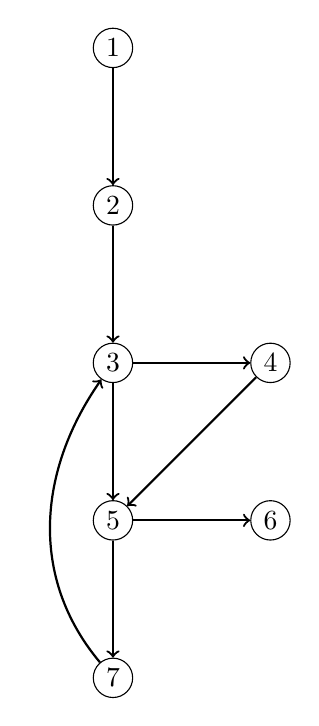
\begin{tikzpicture}[scale=1,place/.style={circle,draw, fill=white,inner sep=0pt,minimum size=5mm}]
        \node (x1)  at (0,0) [place] {1};
        \node (x2)  at (0,-2) [place] {2};
        \node (x3)  at (0,-4) [place] {3};
        \node (x4)  at (2,-4) [place] {4};
        \node (x5)  at (0,-6) [place] {5};
        \node (x6)  at (2,-6) [place] {6};
        \node (x7)  at (0,-8) [place] {7};


        \draw [thick, ->] (x1) -- (x2);
        \draw [thick, ->] (x2) -- (x3);
        \draw [thick, ->] (x3) -- (x4);
        \draw [thick, ->] (x3) -- (x5);
        \draw [thick, ->] (x5) -- (x6);
        \draw [thick, ->] (x5) -- (x7);
        \draw [thick, ->] (x7) to [out=130,in=235] (x3);
        \draw [thick, ->] (x4) -- (x5);
        \end{tikzpicture}
        \label{Fig:7_2_B}
    }
    \caption{一个流程图和它对应的有向图:箭头标注了流程的方向}
    \label{Fig:7_2}
\end{figure*}

\begin{example}
流程图

流程图表示了一个过程内的控制流,或是一个过程中数据或物质的流动。流程图的
框是点;流程图的箭头是边。图\ref{Fig:7_2}以Pascal语法显示了一个例子。
\end{example}

\begin{example}\label{Example:BinRelation}
二元关系

二元关系在\ref{Sec:Relationship}小节中定义。定义R是集合$S={1, \cdots, 10}$上的由
有序对(x,y)组成的二元关系,其中x是y的proper factor;就是说$x\neq y$且$y/x$的
余数是0。回忆$xRy$是$(x,y)\in R$的一种表示。在图\ref{Fig:7_3}的有向图中,
点是S的元素,当且仅当$xRy$时x和y之间有连接边。注意R是传递的:如果$xRy$且$yRz$,则$xRz$。
\end{example}

\begin{figure*}[!t]
    \centering
    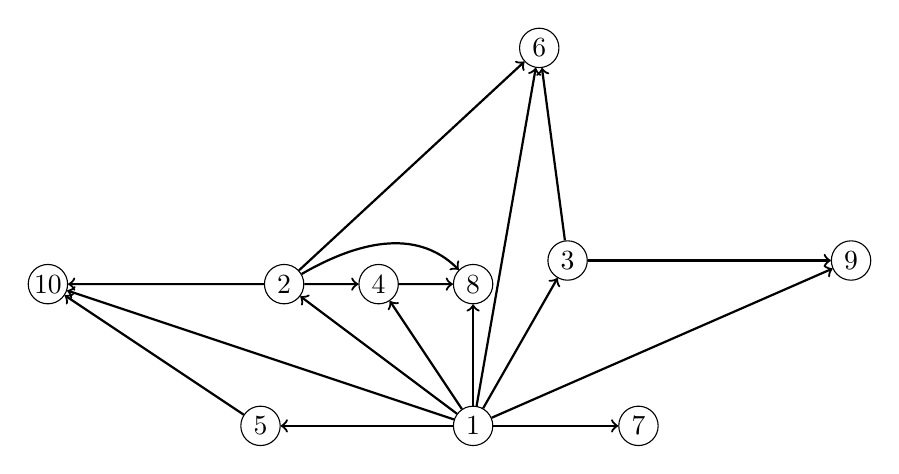
\begin{tikzpicture}[scale=0.6,place/.style={circle,draw, fill=white,inner sep=0pt,minimum size=5mm}]
        \node (x1)  at (0,0) [place] {1};
        \node (x2)  at (-4,3) [place] {2};
        \node (x3)  at (2,3.5) [place] {3};
        \node (x4)  at (-2,3) [place] {4};
        \node (x5)  at (-4.5,0) [place] {5};
        \node (x6)  at (1.4,8) [place] {6};
        \node (x7)  at (3.5,0) [place] {7};
        \node (x8)  at (0,3) [place] {8};
        \node (x9)  at (8,3.5) [place] {9};
        \node (x10)  at (-9,3) [place] {10};

        \draw [thick, ->] (x1) -- (x2);
        \draw [thick, ->] (x1) -- (x3);
        \draw [thick, ->] (x1) -- (x4);
        \draw [thick, ->] (x1) -- (x5);
        \draw [thick, ->] (x1) -- (x6);
        \draw [thick, ->] (x1) -- (x7);
        \draw [thick, ->] (x1) -- (x8);
        \draw [thick, ->] (x1) -- (x9);
        \draw [thick, ->] (x1) -- (x10);
        \draw [thick, ->] (x2) -- (x4);
        \draw [thick, ->] (x2) -- (x6);
        \draw [thick, ->] (x2) to [out=30,in=135] (x8);
        \draw [thick, ->] (x2) -- (x10);
        \draw [thick, ->] (x3) -- (x6);
        \draw [thick, ->] (x3) -- (x9);
        \draw [thick, ->] (x4) -- (x8);
        \draw [thick, ->] (x5) -- (x10);
    \end{tikzpicture}
    \caption{例\ref{Example:BinRelation}中的关系$R$,表示“x是y的proper factor”}
    \label{Fig:7_3}
\end{figure*}

\begin{figure*}[!t]
    \centering
    \subfloat[一个星形网络]{
        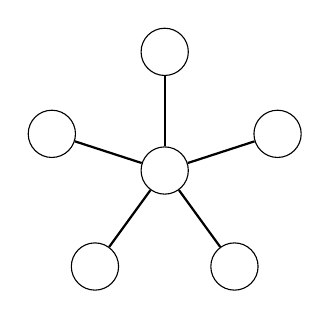
\begin{tikzpicture}[scale=1,place/.style={circle,draw, fill=white,inner sep=0pt,minimum size=6mm}]
            \node[name=s,shape=circle, minimum size=30mm] {};
            \draw[shift=(s.center)]node[name=c,place] {};
            \draw[shift=(s.18)]node[name=x1,place] {};
            \draw[shift=(s.90)]node[name=x2,place] {};
            \draw[shift=(s.162)]node[name=x3,place] {};
            \draw[shift=(s.234)]node[name=x4,place] {};
            \draw[shift=(s.306)]node[name=x5,place] {};

            \draw [thick] (c) -- (x1);
            \draw [thick] (c) -- (x2);
            \draw [thick] (c) -- (x3);
            \draw [thick] (c) -- (x4);
            \draw [thick] (c) -- (x5);
        \end{tikzpicture}
        \label{Fig:7_4_A}
    }
    \hfil
    \subfloat[一个环状网络]{
        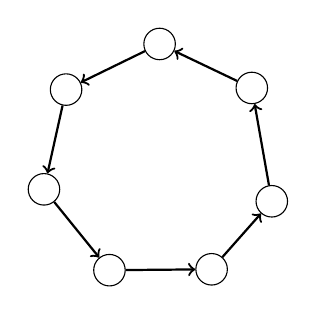
\begin{tikzpicture}[scale=1,place/.style={circle,draw, fill=white,inner sep=0pt,minimum size=4mm}]
            \node[name=s,shape=circle, minimum size=30mm] {};
            \draw[shift=(s.39)]node[name=x1,place] {};
            \draw[shift=(s.90)]node[name=x2,place] {};
            \draw[shift=(s.142)]node[name=x3,place] {};
            \draw[shift=(s.193)]node[name=x4,place] {};
            \draw[shift=(s.245)]node[name=x5,place] {};
            \draw[shift=(s.296)]node[name=x6,place] {};
            \draw[shift=(s.341)]node[name=x7,place] {};

            \draw [thick, ->] (x1) -- (x2);
            \draw [thick, ->] (x2) -- (x3);
            \draw [thick, ->] (x3) -- (x4);
            \draw [thick, ->] (x4) -- (x5);
            \draw [thick, ->] (x5) -- (x6);
            \draw [thick, ->] (x6) -- (x7);
            \draw [thick, ->] (x7) -- (x1);
        \end{tikzpicture}
        \label{Fig:7_4_B}
    }
    \caption{计算机网络}
    \label{Fig:7_4}
\end{figure*}

\begin{example}
计算机网络

点是计算机。线(无向图)或箭头(有向图)是通信线路。图\ref{Fig:7_4}展示
了两个例子。
\end{example}

\begin{example}
集成电路

点可以是二极管、三极管、电容、开关等等。如果两者之间有电路连接则有线。
\end{example}

前面5个例子已经展示了:无向图和有向图提供了一种直接的对分离对象的关系的
抽象形式,包括物理对象和他们的关系(比如,通过航空线路、高速公路和铁路连接
的城市)以及抽象对象的关系(比如二元关系和程序控制结构)。

这些例子同时提出了一些我们可能希望回答的关于所表示的对象以及关系的问题,
这些问题可以转换成图的术语。这样的问题可以通过工作在图上的算法回答。例如,
问题“在San Diego和 Sacramento之间有直通航线吗?”可以转换成“图\ref{Fig:7_1}
中顶点SD和SAC和有边吗?”考虑下面的问题:
\begin{enumerate}
\item 从San Diego飞到Sacramento最便宜的路线是那条?
\item 那条路有最短的飞行时间?
\item 然后一个城市的机场因为坏天气而关闭了,你仍然可以在每对城市之间飞行吗?
\item 如果网络中的一台电脑down掉了,网络中的每对计算机之间还能传递消息吗?
\item 一个点到另一个点之间道路的流量有多大?
\item 一个给定的二元关系是可传递的吗?
\item 给定一个流程图有循环吗?
\item 如何连接不同的电路端口使得连接所有的需要的电线最少?
\end{enumerate}
本章和下面的章中我们将学习算法回答大多数问题。

\subsection{基本的图定义}
本小节主要是图的定义和基本注意。许多申明和定义都同时适用于有向和无向图,
我们使用公用的符号表示两者共同的部分。当然,无向和有向图不一样的部分我们
将特别注明。

\begin{definition}
有向图

一个\emph{有向图或digraph}是一个pair $G=(V,E)$,这里$V$是一个集合,它
的元素是\emph{顶点},$E$也是一个集合它的元素是$V$元素的有序对。顶点通常也叫
\emph{节点}。E的元素叫\emph{边},或是\emph{有向边},或是弧。对于$E$中的
有向边$(v, w)$,$v$叫做尾,$w$叫做头;$(v,w)$表示为一个有向箭头$v \rightarrow w$。
在文本中我们简单的写作$vw$。
\end{definition}

在二元关系例子中(例\ref{Example:BinRelation},图\ref{Fig:7_3}),
\begin{displaymath}
\begin{aligned}
&V=\{1,2, \cdots, 10\}\\
&E=\{(1,2), \cdots, (1,10), (2,4),(2,6), (2,8),
(2,10),(3,6),(3,9),(4,8),(5,10)\}
\end{aligned}
\end{displaymath}

\begin{definition}
无向图

一个\emph{无向图graph}是一个pair $G=(V,E)$,这里$V$是一个集合,它
的元素是\emph{顶点},$E$也是一个集合它的元素是$V$元素的无序对。顶点通常也叫
\emph{节点}。E的元素叫\emph{边},或是为了强调叫做\emph{无向边}。每一个边都
可以认为是包含两个元素$V$的子集;因此符号${v, w}$表示无向边。用v-w表示。在文本
中我们简单的写作$vw$。当然对于无向图$wv=vw$。
\end{definition}

例如对于例子\ref{Example:AirRouteMap}和图\ref{Fig:7_1},我们有
\begin{displaymath}
\begin{aligned}
&V=\{SF,OAK, SAC, STK, FRES, LA, SD\}\\
&E=\{(SF,STK), (SF,SAC), (SF,LA),(SF,SD), (SF,FRES),\\
&(SD,OAK),(SAC,LA),(LA,OAK),(LA,FRES),\\
&(LA,SD),(FRES, STK), (SD, FRES)\}
\end{aligned}
\end{displaymath}
无向图的定义暗示了不存在连接顶点自己的图:边定义为包含两个元素,一个集合
不能有重复的元素(\ref{Sec:SetTupleRelation}小节)。

\begin{definition}
子图,对称图,完全图

一个图$G=(V,E)$的子图$G'=(V',E'),V'\subseteq V, E'\subseteq
E$。由图的定义 还需要满足$E' \subseteq  V'\times V'$.

对称图是这样的有向图:有边$vw$则必有反方向边$wv$.每个无向图有对应的对称图,把
无向边解释成相反方向的一对有向边.

完全图(正常是无向图)是每对顶点都有边的图.

边$vw$可说它是依附于顶点$v$和$w$的.
\end{definition}

\begin{definition}
邻接关系

图或有向图$G=(V,E)$的边引出了一种在顶点集合上的关系A,称之为\emph{邻接关系}。
令$v$和$w$是$V$的元素。则$vAw$(读作“$w$是$v$的邻接”)当且仅当$vw$在$E$
中。换句话说,$vAw$意味着可以从$v$出发通过$G$的边到达$w$。如果$G$是无向图,
关系是A是对称的。(就是说$wAv$当且仅当$vAw$。)
\end{definition}

路径path的概念在许多应用中非常有用,包括那些牵涉到人、电话(或者电子)消息、
手机漫游、管道中的油和气等等的route问题,以及其他路径表示抽象的属性的问题
(参看练习7.3)。再次考虑\ref{Fig:7_1},假设我们希望做飞机从Los Angeles(LA)
到Fresno(FRES)。有一条边\{LA, FRES\}是可能的路由,但是也有其他的。我们可以
从LA到SAC到SF到FRES,或者我们可以从LA到SD到FRES。图中LA到FRES的都称为“路径”。

\begin{definition}\label{Def:PathinGraph}
图中路径

图$G=(V,E)$中一条\emph{从v到w路径}是边$v_0v_1, v_1v_2, \cdots, v_{k-1}vk$的
序列,这里$v=v_0$和$v_k =w$。路径的长度是$k$。一个孤立顶点$v$可以认为是一条
长度为0的自己到自己的路径。一条\emph{简单路径}指$v_0, v_1, \cdots, v_k$都是
不同。

说一个顶点$w$从$v$\emph{可到达},当从$v$到$w$有一条路径。
\end{definition}

\begin{figure*}[!t]
    \centering
    \begin{tikzpicture}[scale=0.8,place/.style={shape=ellipse,draw, fill=white,inner sep=0pt,minimum width=10ex,minimum height=5ex}]
        \node (SAC)  at (2,11) [place] {SAC};
        \node (SF)  at (-2.4,9.7) [place] {SF};
        \node (STK)  at (4.6,10) [place] {STK};
        \node (OAK)  at (-0.4,9) [place] {OAK};
        \node (FRES)  at (3,5) [place] {FRES};
        \node (LA)  at (-1.4,1) [place] {LA};
        \node (SD)  at (0,0) [place] {SD};

        \draw [ultra thick] (SAC) -- (SF);
        \draw [thick] (SF) -- (STK);
        \draw [thick] (SF) -- (LA);
        \draw [thick] (SF) -- (SD);
        \draw [ultra thick] (SF) -- (FRES);
        \draw [thick] (LA) -- (OAK);
        \draw [thick] (LA) -- (FRES);
        \draw [thick] (LA) -- (SD);
        \draw [ultra thick] (SD) -- (FRES);
        \draw [thick] (LA) -- (SAC);
        \draw [thick] (STK) -- (FRES);
        \draw [thick] (SD) -- (OAK);
        \end{tikzpicture}
    \caption{SD到SAC的路径}
    \label{Fig:7_5}
\end{figure*}

路径\{SD, FRES\}, \{FRES, SF\}, \{SF, SAC\}展示在图\ref{Fig:7_5}。我们通
列出路径穿过的所有顶点来标注一条路径(但是记住路径的长度是它穿过的边的
数量)。因此在图\ref{Fig:7_5}是SD,FRES,SD,SAC,长度是3。

\begin{definition}
连通,强连通

\emph{连通性connectivity}的定义需要特别注意,因为有向图的连通性和无向图的
连通性有区别。

无向图的是\emph{连同}的,当且仅当对于每一对顶点$v$和$w$都存在一条路径从
$v$到$w$。

有向图的是强联通的,当且仅当对于每一对顶点$v$和$w$都存在一条路径从$v$到$w$。
\end{definition}

分成两个读起来差不多的独立定义的原因是,在无向图中,如果存在从$v$到$w$的路径
则自动存在从$w$到$v$的路径。在有向图中,这就不一定是真,因此限定词“强”用来
表示条件是强的。如果我们将无向图视为双向街道系统,将有向图视为单向街道系统,
则强连通性意味着我们可以从一点到任意一点,即使沿着单行街道的单行方向。这显然
是比双向街道更严格的条件。

\begin{definition}
图中的回路cycle in graph

\emph{回路}的定义需要特别注意,因为有向图的回路和无向图的回路有区别。

对于有向图,一条\emph{回路}仅是一条非空的路径,也就是路径的起始顶点是一样,
一条\emph{简单回路}是一条顶点不重复的回路,除了起始顶点是一样的。

对于有向图定义是类似的,但是增加了要求:如果同一条边出现超过一次,它总是
以同样的方向出现。就是说,使用定义\ref{Def:PathinGraph}的标记表示,如果$v_i=x$
和$v_{i+1}=y$其中$0\leq i <k$,则不存在$j$使得$v_j=y$且$v_{j+1}=x$。

一个图是\emph{无环的acyclic},如果它没有回路。

一个\emph{无环无向图}叫\emph{无向森林}。如果图还是联通的,它是\emph{自由树},
或\emph{无向树}。

一个\emph{有向}无环图通常简写为\emph{DAG}。(一个DAG并不假设满足任何连通性
条件。)
\end{definition}

\begin{figure*}[!t]
    \centering
    \begin{tikzpicture}[scale=1,place/.style={minimum height=2ex}]
        \node (c1)  at (0,0) [place] {C};
        \node (c2)  at (1,0) [place] {C};
        \node (h1)  at (-1,0) [place] {H};
        \node (h2)  at (0,1) [place] {H};
        \node (h3)  at (0,-1) [place] {H};
        \node (h4)  at (1,1) [place] {H};
        \node (h5)  at (1,-1) [place] {H};
        \node (h6)  at (3,0) [place] {H};
        \node (o1)  at (2,0) [place] {O};

        \draw [] (c1) -- (h1);
        \draw [] (c1) -- (h2);
        \draw [] (c1) -- (h3);
        \draw [] (c1) -- (c2);
        \draw [] (c2) -- (h4);
        \draw [] (c2) -- (h5);
        \draw [] (c2) -- (o1);
        \draw [] (o1) -- (h6);
        \end{tikzpicture}
    \caption{自由树,表示酒精的分子式}
    \label{Fig:7_6}
\end{figure*}

图\ref{Fig:7_6}是一个自由,或无向树。注意根据树的定义,没有顶点被选作根。一颗
\emph{rooted tree}是一颗树,它有一个顶点设计成了根。一旦根指定之后,树常用的
父子关系就可以派生出来。

定义\emph{对称有向图}和\emph{对称无向图}的原因牵涉到回路。如果回路的概念不重要,
则a procedure intended for directed graphs can often be used on the 对称有向图
that corresponds to an undirected graph. 但是对于那些回路概念很重要的问题,这种
代入并不好用。例如,简单的无向图有一条边$ab$,且没有回路,但是它的对称对应图有
两条边$ab$和$ba$,且有一个回路。

\begin{definition}\label{Def:Connected_Component}
连同分量connected component

无向图$G$的\emph{连同分量}是$G$的\emph{最大}连同子图,相关概念很多,它的定义
延缓到定义\ref{Def:CondensationGraph}。
\end{definition}

我们必须澄清连同分量中“最大”的含义。说一个图在某些图的集合中是\emph{最大的},
当它不是集合中任意图的真子图。它不需要有在图集合中最多的顶点数或者最多的边数。
在定义\ref{Def:Connected_Component}中,“集合collection”是$G$中所有连同子图。

当术语\emph{分量}用于图的连同时和其他抽象结构时,它通常隐含包括了在组中的最大性。
我们将在本章的后面遇到术语“强连同分量”和“二连同分量”。两种情况中都有最大性
的概念。

\begin{figure*}[!t]
    \centering
    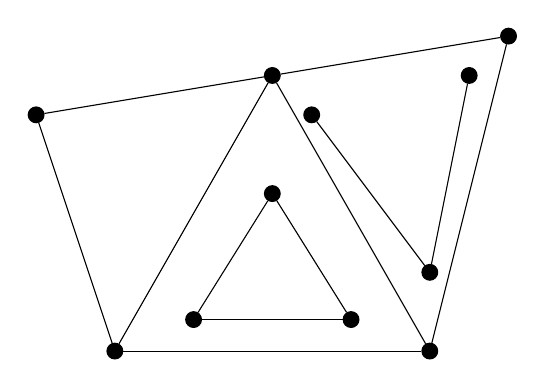
\begin{tikzpicture}[scale=1,place/.style={circle,draw, fill=black,inner sep=0pt,minimum size=2mm}]
        \node (x1) at (0,0) [place] {};
        \node (x2) at (3,0.5) [place] {};
        \node (x3) at (6,1) [place] {};
        \node (x5) at (1,-3) [place] {};
        \node (x6) at (5,-3) [place] {};
        \node (x7) at (2,-2.6) [place] {};
        \node (x8) at (4,-2.6) [place] {};
        \node (x4) at (3,-1) [place] {};
        \node (x9) at (3.5,0) [place] {};
        \node (x10) at (5.5,0.5) [place] {};
        \node (x11) at (5,-2) [place] {};

        \draw [] (x1)-- (x2);
        \draw [] (x2)--(x3);
        \draw [] (x1)-- (x5);
        \draw [] (x3)--(x6);
        \draw [] (x5)-- (x6);
        \draw [] (x2)--(x6);
        \draw [] (x2)--(x5);
        \draw [] (x7)-- (x8);
        \draw [] (x8)--(x4);
        \draw [] (x4)--(x7);
        \draw [] (x9)--(x11);
        \draw [] (x10)--(x11);

    \end{tikzpicture}
    \caption{有三个连同分量的图}
    \label{Fig:7_7}
\end{figure*}

如果无向图不是连同的,它可以划分为独立的连同分量,且这个划分是唯一的。图
\ref{Fig:7_7}有三个连同分量。

\begin{figure*}[!t]
    \centering
    \begin{tikzpicture}[scale=0.8,place/.style={shape=ellipse,draw, fill=white,inner sep=0pt,minimum width=10ex,minimum height=5ex}]
        \node (SAC)  at (2,11) [place] {SAC};
        \node (SF)  at (-2.4,9.7) [place] {SF};
        \node (STK)  at (4.6,10) [place] {STK};
        \node (OAK)  at (-0.4,9) [place] {OAK};
        \node (FRES)  at (3,5) [place] {FRES};
        \node (LA)  at (-1.4,1) [place] {LA};
        \node (SD)  at (0,0) [place] {SD};

        \draw [ultra thick] (SAC) -- (SF)node[above,text centered,midway]{48};
        \draw [thick] (SF) -- (STK)node[above,text centered,midway]{48};
        \draw [thick] (SF) -- (LA)node[left,text centered,midway]{100};
        \draw [thick] (SF) -- (SD)node[above,text centered,midway]{128};
        \draw [ultra thick] (SF) -- (FRES)node[above,text centered,midway]{64};
        \draw [thick] (LA) -- (OAK)node[above,text centered,midway]{100};
        \draw [thick] (LA) -- (FRES)node[above,text centered,midway]{80};
        \draw [thick] (LA) -- (SD)node[above,text centered,midway]{48};
        \draw [ultra thick] (SD) -- (FRES)node[above,text centered,midway]{120};
        \draw [thick] (LA) -- (SAC)node[above,text centered,midway]{100};
        \draw [thick] (STK) -- (FRES)node[right,text centered,midway]{48};
        \draw [thick] (SD) -- (OAK)node[right,text centered,midway]{128};
        \end{tikzpicture}
    \caption{图的权值表示了票价}
    \label{Fig:7_8}
\end{figure*}

在许多图的应用中很自然的为每条边关联到一个数字,通常成为\emph{权值weight}。
数字表示以某种方式使用边带来的消耗或者收益。再次考虑图\ref{Fig:7_1},假设
我们想从SD飞到SAC。有一个不停站飞行,但是可以使用好几种route和路径。那种
最好?为了回答这个问题,我们需要一个比较不同路径的标准。可能的标准有
\begin{enumerate}
\item 中途停的次数
\item 总的票价
\item 总的飞行时间
\end{enumerate}
在选择了标准之后,我们可以赋值给每一条边一个值,代表通过这条边旅行的消耗
(停的次数,钱或时间)。一条特定路径的总消耗是这条route遍历到所有边消耗
的和。图\ref{Fig:7_8}展示的航空图(假象的)上带上了每条边机票的价格。你
可以验证最便宜的从SD到SAC的方式是在LA中转一次。寻找“最好”路径的一般性
问题在\ref{Sec:single-source-shortest-path}节和\ref{Sec:AllParisShortestPathsinGraphs}
节学习。

\begin{figure*}[!t]
    \centering
    \begin{tikzpicture}[scale=1,place/.style={circle,draw, fill=black,inner sep=0pt,minimum size=2mm}]
        \node (x1) at (0,0) [place] {};
        \node (x2) at (12,1) [place] {};
        \draw [] (x1) -- (x2)
            node[above, text centered, midway]{20};

        \node (xa1) at (-0.2,1) [place] {};
        \node (xb1) at (-1.2,0) [place] {};
        \draw [] (x1) -- (xa1)
            node[above, text centered, midway]{18};
        \draw [] (x1) -- (xb1)
            node[above, text centered, midway]{20};

        \node (xa2) at (12.2,2) [place] {};
        \node (xb2) at (13.2,-0.1) [place] {};
        \draw [] (x2) -- (xa2)
            node[above, text centered, midway]{15};
        \draw [] (x2) -- (xb2)
            node[above, text centered, midway]{20};

        \node (x3) at (0.3,-1) [place] {};
        \draw [] (x1) -- (x3)
            node[above, text centered, midway]{18};

        \node (x4) at (0.6,-2.3) [place] {};
        \draw [] (x3) -- (x4)
            node[above, text centered, midway]{18};

        \node (x5) at (0.9,-3.6) [place] {};
        \draw [] (x4) -- (x5)
            node[above, text centered, midway]{18};
        \node (xa5) at (-0.6,-3.6) [place] {};
        \draw [] (x5) -- (xa5)
            node[above, text centered, midway]{10};

        \node (x6) at (1.9,-7.4) [place] {};
        \draw [] (x5) -- (x6)
            node[above, text centered, midway]{18};
        \node (xa6) at (-0.3,-8.0) [place] {};
        \draw [] (x6) -- (xa6)
            node[above, text centered, midway]{6};

        \node (x7) at (2.6,-10) [place] {};
        \draw [] (x6) -- (x7)
            node[above, text centered, midway]{18};


    \end{tikzpicture}
    \caption{显示交通能力的街道地图}
    \label{Fig:7_9}
\end{figure*}

图\ref{Fig:7_9}\footnote{译注:对原图有简化},展示了城市中的一些街道,可能被
用于自动交通流的研究。赋予边的数字指示了交通的量,即相同时间间隔内能通过街道
的流量。数字取决于路的类型和大小,速度限制,两个街区之间交通灯的数量,街区在
图中以顶点指示(假设不是所有的街道都显示在途中),以及其他的因素。

The assignment of numbers of edges occurs often enough in applications to
merit a definition.

\begin{definition}
带权图

带权图是一个三元组$(V,E,W)$,这里$(V,E)$是图(有向或者无向图)而$W$是一个
E到$\mathbf{R}$(实数)的函数。(其他权的类型,比如有理数或整数,可以适用与
有些问题。)对于边$e$,$W(e)$叫$e$的\emph{权值}。
\end{definition}

函数这个术语可能听起来很技术化,但是只要我们回顾\ref{Sec:Calculous}小节就很容易
理解,概念上,函数仅仅是一张双列的表:函数的参数和参数对应的函数的值。这种情况
下每条边表示在第一列中的某一行,它的权值在第二列中同样的行中。数据结构表示上
可能会不同,但是权值代表着同样的信息。在图的图形表示中,我们简单的将每条边的权
写在边的旁边,就像我们在图\ref{Fig:7_8}和\ref{Fig:7_9}。在有些应用中权将表示消耗
或者其他边的负面东西,而有些问题中权是能力或者边的有益属性。(随着应用的不同;
因此术语\emph{cost}, \emph{length}, or \emph{capacity} 可以替代为\emph{weight}。)
在许多应用中,权不能自然认为是负的,as when 他们表示距离时。有些算法的正确性
依赖严格的权值的非负性,而有些算法能处理负值。


\subsection{图的表示和数据结构}\label{Sec:GraphRepresentationsAndDataStructures}
我们有两种在纸上表示图的方法:画张图片,图片中顶点用点表示,边用线或者箭头表示;
列出顶点和边。这一小节讨论通常在计算机程序中用来表示图的数据结构。令$G=(V,E)$是图,
其中$n=|V|$, $m=|E|$, 和$V={v_1, v_2, \cdots, v_n}$。

\subsubsection{邻接矩阵}
\begin{figure*}[!t]
    \centering
    \subfloat[一个无向图]{
        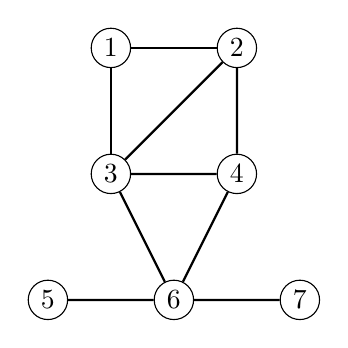
\begin{tikzpicture}[scale=0.8,place/.style={circle,draw, fill=white,inner sep=0pt,minimum size=5mm}]
        \node (x1)  at (0,0) [place] {1};
        \node (x2)  at (2,0) [place] {2};
        \node (x3)  at (0,-2) [place] {3};
        \node (x4)  at (2,-2) [place] {4};
        \node (x5)  at (-1,-4) [place] {5};
        \node (x6)  at (1,-4) [place] {6};
        \node (x7)  at (3,-4) [place] {7};

        \draw [thick] (x1) -- (x2)
            node[right,text centered,midway]{};
        \draw [thick] (x2) -- (x3)
            node[above,text centered,midway]{};
        \draw [thick] (x2) -- (x4)
            node[left,text centered,midway]{};
        \draw [thick] (x3) -- (x1)
            node[above,text centered,midway]{};
        \draw [thick] (x3) -- (x6)
            node[text centered,midway]{};
        \draw [thick] (x4) -- (x3)
            node[text centered,midway]{};
        \draw [thick] (x6) -- (x5)
            node[text centered,midway]{};
        \draw [thick] (x6) -- (x4)
            node[text centered,midway]{};
        \draw [thick] (x7) -- (x6)
            node[text centered,midway]{};
        \end{tikzpicture}
        \label{Fig:7_10_A}
    }
    \hfil
    \subfloat[它的邻接矩阵]{
        $\left(
           \begin{array}{ccccccc}
             0 & 1 & 1 & 0 & 0 & 0 & 0 \\
             1 & 0 & 1 & 1 & 0 & 0 & 0 \\
             1 & 1 & 0 & 1 & 0 & 1 & 0 \\
             0 & 1 & 1 & 0 & 0 & 1 & 0 \\
             0 & 0 & 0 & 0 & 0 & 1 & 0 \\
             0 & 0 & 1 & 1 & 1 & 0 & 1 \\
             0 & 0 & 0 & 0 & 0 & 1 & 0 \\
           \end{array}
         \right)
        $
        \label{Fig:7_10_B}
    }
    \hfil
    \subfloat[它的邻接表结构]{
        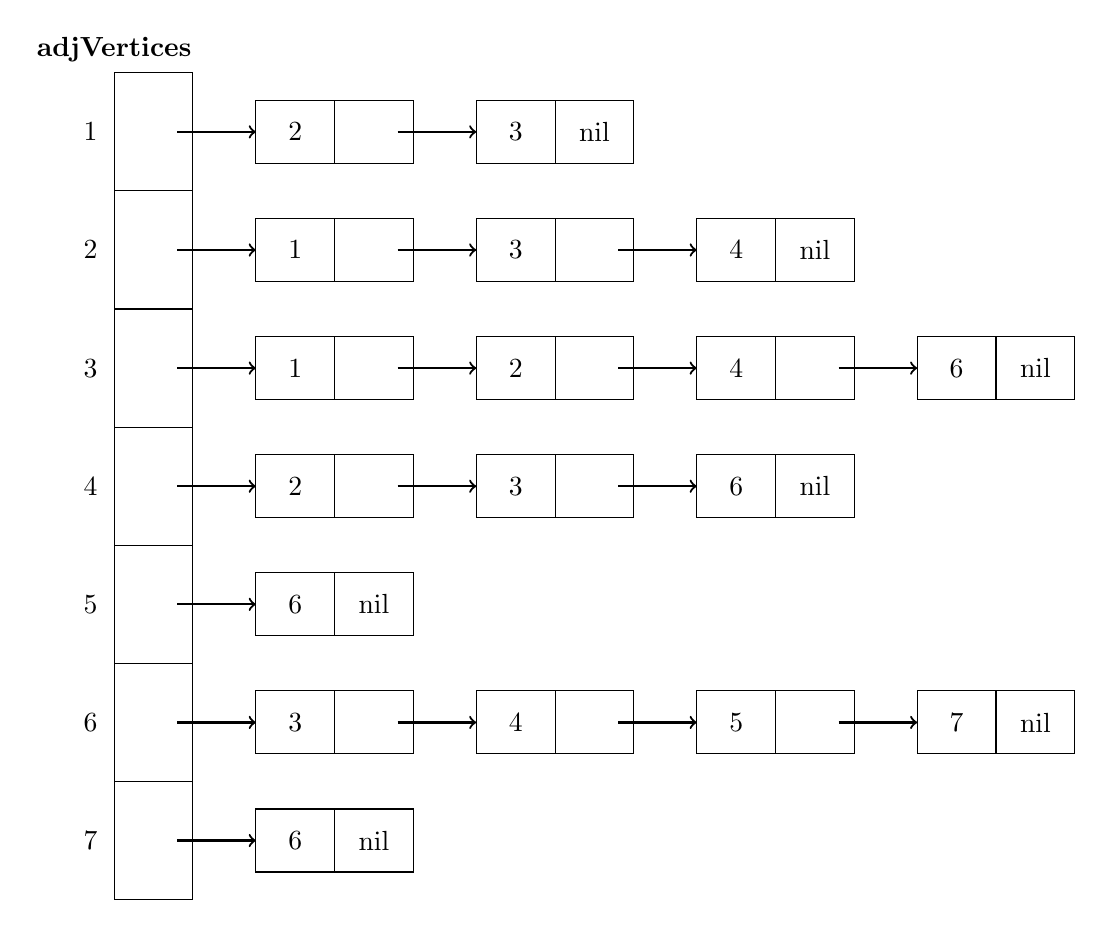
\begin{tikzpicture}[scale=1,place/.style={circle,draw, fill=white,inner sep=0pt,minimum size=5mm}]
        \draw (0, 0.3) node{{\textbf{adjVertices}}};
        \foreach \x in {1, ..., 7}
            \draw (-0.3, -\x*1.5+0.75) node{\x};
        \foreach \x in {1, ..., 7}
            \draw (0,-\x*1.5) rectangle (1,-\x*1.5+1.5);
        \foreach \x in {1, ..., 7}
            \draw [thick, ->] (0.8,-\x*1.5+0.75) -- (1.8,-\x*1.5+0.75);
        \foreach \x in {1, ..., 7}
            \draw (1.8, -\x*1.5+0.75-0.4) rectangle (2.8,-\x*1.5+0.75+0.4);
        \foreach \x in {1, ..., 7}
            \draw (2.8, -\x*1.5+0.75-0.4) rectangle (3.8,-\x*1.5+0.75+0.4);
        \foreach \x/\y in {1/2, 2/1, 3/1, 4/2, 5/6, 6/3, 7/6}
            \draw (2.3, -\x*1.5+0.75) node {\y};
        \foreach \x/\y in {5/nil, 7/nil}
            \draw (3.3, -\x*1.5+0.75) node {\y};

        \foreach \x in {1, 2, 3, 4, 6}
            \draw [thick, ->] (3.6,-\x*1.5+0.75) -- (4.6,-\x*1.5+0.75);
        \foreach \x in {1, 2, 3, 4, 6}
            \draw (4.6, -\x*1.5+0.75-0.4) rectangle (5.6,-\x*1.5+0.75+0.4);
        \foreach \x in {1, 2, 3, 4, 6}
            \draw (5.6, -\x*1.5+0.75-0.4) rectangle (6.6,-\x*1.5+0.75+0.4);
        \foreach \x/\y in {1/3, 2/3, 3/2, 4/3, 6/4}
            \draw (5.1, -\x*1.5+0.75) node {\y};
        \foreach \x/\y in {1/nil}
            \draw (6.1, -\x*1.5+0.75) node {\y};

        \foreach \x in {2, 3, 4, 6}
            \draw [thick, ->] (6.4,-\x*1.5+0.75) -- (7.4,-\x*1.5+0.75);
        \foreach \x in {2, 3, 4, 6}
            \draw (7.4, -\x*1.5+0.75-0.4) rectangle (8.4,-\x*1.5+0.75+0.4);
        \foreach \x in {2, 3, 4, 6}
            \draw (8.4, -\x*1.5+0.75-0.4) rectangle (9.4,-\x*1.5+0.75+0.4);
        \foreach \x/\y in {2/4, 3/4, 4/6, 6/5}
            \draw (7.9, -\x*1.5+0.75) node {\y};
        \foreach \x/\y in {2/nil, 4/nil}
            \draw (8.9, -\x*1.5+0.75) node {\y};

        \foreach \x in {3, 6}
            \draw [thick, ->] (9.2,-\x*1.5+0.75) -- (10.2,-\x*1.5+0.75);
        \foreach \x in {3, 6}
            \draw (10.2, -\x*1.5+0.75-0.4) rectangle (11.2,-\x*1.5+0.75+0.4);
        \foreach \x in {3, 6}
            \draw (11.2, -\x*1.5+0.75-0.4) rectangle (12.2,-\x*1.5+0.75+0.4);
        \foreach \x/\y in {3/6, 6/7}
            \draw (10.7, -\x*1.5+0.75) node {\y};
        \foreach \x/\y in {3/nil, 6/nil}
            \draw (11.7, -\x*1.5+0.75) node {\y};

        \end{tikzpicture}
        \label{Fig:7_10_C}
    }
    \caption{边不带权的无向图的两种表示,邻接矩阵和邻接表。它也可以是一个对称有向图。}
    \label{Fig:7_10}
\end{figure*}

\begin{figure*}[!t]
    \centering
    \subfloat[一个带权有向图]{
        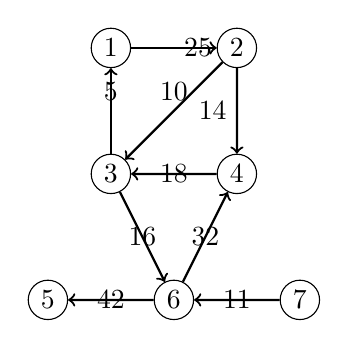
\begin{tikzpicture}[scale=0.8,place/.style={circle,draw, fill=white,inner sep=0pt,minimum size=5mm}]
        \node (x1)  at (0,0) [place] {1};
        \node (x2)  at (2,0) [place] {2};
        \node (x3)  at (0,-2) [place] {3};
        \node (x4)  at (2,-2) [place] {4};
        \node (x5)  at (-1,-4) [place] {5};
        \node (x6)  at (1,-4) [place] {6};
        \node (x7)  at (3,-4) [place] {7};

        \draw [thick, ->] (x1) -- (x2)
            node[right,text centered,midway]{25};
        \draw [thick, ->] (x2) -- (x3)
            node[above,text centered,midway]{10};
        \draw [thick, ->] (x2) -- (x4)
            node[left,text centered,midway]{14};
        \draw [thick, ->] (x3) -- (x1)
            node[above,text centered,midway]{5};
        \draw [thick, ->] (x3) -- (x6)
            node[text centered,midway]{16};
        \draw [thick, ->] (x4) -- (x3)
            node[text centered,midway]{18};
        \draw [thick, ->] (x6) -- (x5)
            node[text centered,midway]{42};
        \draw [thick, ->] (x6) -- (x4)
            node[text centered,midway]{32};
        \draw [thick, ->] (x7) -- (x6)
            node[text centered,midway]{11};
        \end{tikzpicture}
        \label{Fig:7_11_A}
    }
    \hfil
    \subfloat[它的邻接矩阵]{
        $\left(
           \begin{array}{ccccccc}
             0 & 25.0 & \infty & \infty & \infty & \infty & \infty \\
             \infty & 0 & 10.0 & 14.0 & \infty & \infty & \infty \\
             5.0 & \infty & 0 & \infty & \infty & 16.0 & \infty \\
             \infty & 6.0 & 18.0 & 0 & \infty & \infty & \infty \\
             \infty & \infty & \infty & \infty & 0 & \infty & \infty \\
             \infty & \infty & \infty & 32.0 & 42.0 & 0 & 14.0 \\
             \infty & \infty & \infty & \infty & \infty & 11.0 & 0 \\
           \end{array}
         \right)
        $
        \label{Fig:7_11_B}
    }
    \hfil
    \subfloat[它的邻接表结构]{
        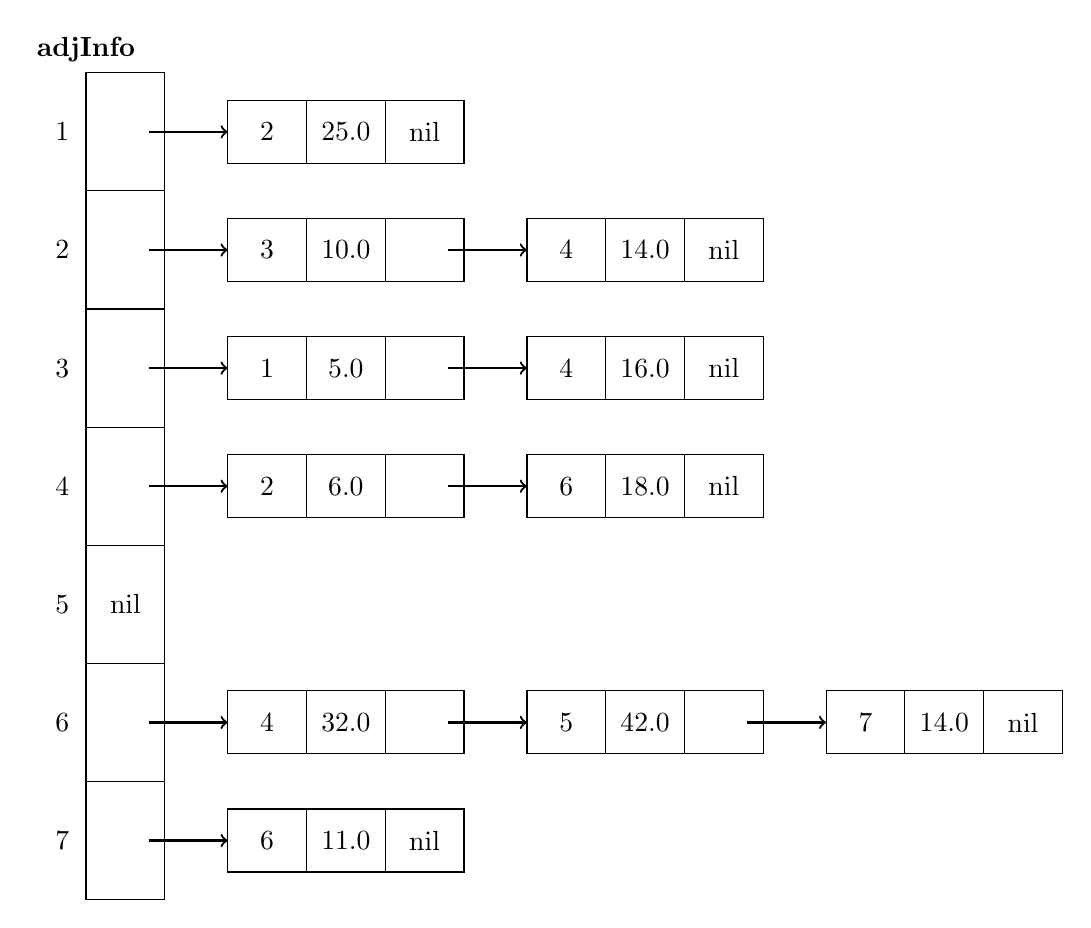
\begin{tikzpicture}[scale=1,place/.style={circle,draw, fill=white,inner sep=0pt,minimum size=5mm}]
        \draw (0, 0.3) node{{\textbf{adjInfo}}};
        \foreach \x in {1, ..., 7}
            \draw (-0.3, -\x*1.5+0.75) node{\x};
        \foreach \x in {1, ..., 7}
            \draw (0,-\x*1.5) rectangle (1,-\x*1.5+1.5);
        \foreach \x/\y in {5/nil}
            \draw (0.5, -\x*1.5+0.75) node {\y};

        \foreach \x in {1, ..., 4, 6, 7}
            \draw [thick, ->] (0.8,-\x*1.5+0.75) -- (1.8,-\x*1.5+0.75);
        \foreach \x in {1, ..., 4, 6, 7}
            \draw (1.8, -\x*1.5+0.75-0.4) rectangle (2.8,-\x*1.5+0.75+0.4);
        \foreach \x in {1, ..., 4, 6, 7}
            \draw (2.8, -\x*1.5+0.75-0.4) rectangle (3.8,-\x*1.5+0.75+0.4);
        \foreach \x in {1, ..., 4, 6, 7}
            \draw (3.8, -\x*1.5+0.75-0.4) rectangle (4.8,-\x*1.5+0.75+0.4);
        \foreach \x/\y in {1/2, 2/3, 3/1, 4/2, 6/4, 7/6}
            \draw (2.3, -\x*1.5+0.75) node {\y};
        \foreach \x/\y in {1/25.0, 2/10.0, 3/5.0, 4/6.0, 6/32.0, 7/11.0}
            \draw (3.3, -\x*1.5+0.75) node {\y};
        \foreach \x/\y in {1/nil, 7/nil}
            \draw (4.3, -\x*1.5+0.75) node {\y};

        \foreach \x in {2, 3, 4, 6}
            \draw [thick, ->] (4.6,-\x*1.5+0.75) -- (5.6,-\x*1.5+0.75);
        \foreach \x in {2, 3, 4, 6}
            \draw (5.6, -\x*1.5+0.75-0.4) rectangle (6.6,-\x*1.5+0.75+0.4);
        \foreach \x in {2, 3, 4, 6}
            \draw (6.6, -\x*1.5+0.75-0.4) rectangle (7.6,-\x*1.5+0.75+0.4);
        \foreach \x in {2, 3, 4, 6}
            \draw (7.6, -\x*1.5+0.75-0.4) rectangle (8.6,-\x*1.5+0.75+0.4);
        \foreach \x/\y in {2/4, 3/4, 4/6, 6/5}
            \draw (6.1, -\x*1.5+0.75) node {\y};
        \foreach \x/\y in {2/14.0, 3/16.0, 4/18.0, 6/42.0}
            \draw (7.1, -\x*1.5+0.75) node {\y};
        \foreach \x/\y in {2/nil, 3/nil, 4/nil}
            \draw (8.1, -\x*1.5+0.75) node {\y};

        \foreach \x in {6}
            \draw [thick, ->] (8.4,-\x*1.5+0.75) -- (9.4,-\x*1.5+0.75);
        \foreach \x in {6}
            \draw (9.4, -\x*1.5+0.75-0.4) rectangle (10.4,-\x*1.5+0.75+0.4);
        \foreach \x in {6}
            \draw (10.4, -\x*1.5+0.75-0.4) rectangle (11.4,-\x*1.5+0.75+0.4);
        \foreach \x in {6}
            \draw (11.4, -\x*1.5+0.75-0.4) rectangle (12.4,-\x*1.5+0.75+0.4);
        \foreach \x/\y in { 6/7}
            \draw (9.9, -\x*1.5+0.75) node {\y};
        \foreach \x/\y in {6/14.0}
            \draw (10.9, -\x*1.5+0.75) node {\y};
        \foreach \x/\y in {6/nil}
            \draw (11.9, -\x*1.5+0.75) node {\y};
        \end{tikzpicture}
        \label{Fig:7_11_C}
    }
    \caption{带权有向图的两种表示。}
    \label{Fig:7_11}
\end{figure*}

$G$可以表示为$n\times n$矩阵$A=(a_{ij})$,称为$G$的\emph{邻接矩阵}。A定义为
\begin{displaymath}
a_{ij}=\left\{\begin{array}{l}
                   1 \qquad\mbox{if } v_iv_j \in E\\
                   \raggedleft 0 \qquad\mbox{otherwise}
                 \end{array}
\right.\qquad\mbox{for }1\leq i, j\leq n.
\end{displaymath}
无向图的邻接矩阵是对称的(仅有一半需要存储)。如果$G=(V,E,W)$是带权图,权可以
存储在邻接矩阵中,只需改动一下定义:
\begin{displaymath}
\begin{aligned}
a_{ij}=\left\{\begin{array}{ll}
                   W(v_iv_j) &\mbox{if } v_iv_j \in E\\
                   c &\mbox{otherwise}
                 \end{array}
\right.\qquad\mbox{for }1\leq i, j\leq n.
\end{aligned}
\end{displaymath}
这里\emph{c}常数,它的值以来与权的实现以及要解决的问题。如果权是一种消耗,$c$
可以选择$\infty$(或者其他特别大的数)因为遍历不存在的边的消耗可能高的惊人。
如果权是能力,选择$c=0$通常是合适的,因为不存在的边不会有任何效果。 参看
图\ref{Fig:7_10_A},\ref{Fig:7_10_B}和\ref{Fig:7_11_A},\ref{Fig:7_11_B}。

有些在图上解决问题的算法需要检查每一条边并且以某种方式处理边一次。如果使用
邻接矩阵的表示,我们可以把graph想像成每一对顶点之间都有边,因为许多算法将会
检查矩阵的每一个条目以判断这条边是否存在。既然有向图中边可能的数量是$n^2$,或者
无向图是$n(n-1)/2$,这样的算法的复杂性在$\Omega(n^2))$。

\subsubsection{邻接表数组}
邻接矩阵表示之外另一种方法是用顶点的编号来索引的数组,数组中包含了链表,称之为
\emph{邻接表(adjacency lists)}。对于每一个顶点$v_i$,第$i$个数组元素包含一个
list,list中是图$G$中所有从$v_i$出发的边的信息。在有向图中,这意味着$v_i$是边的
尾;在无向图中,边是关联到$v_i$的。$v_i$的list包含每条边的一个元素。为了确定性
的表述,我们称这个数组是{\textbf{adjInfo}}。它有以下定义:
\begin{lstlisting}[language={Java}, keywordstyle=\color{blue!70}, commentstyle=\color{red!50!green!50!blue!50}]
    List[] adjInfo = new List[n+1];
\end{lstlisting}
我们将使用索引$1,\cdots, n$,所以我们分配了$n+1$个位置,但是不使用第0个位置。
现在adjInfo[i]将是一个list,list中包含从$v_i$出发的边的信息。

邻接表结构的长处是,$G$中不存在的边也不会存在于我们的数据结构中。如果$G$是
稀疏的(包含的边远小于$n^2$),邻接表处理起来比较迅速。注意,如果邻接表中的元素
以不同的顺序出现,邻接表结构依然表示的是同一个图,但是使用list的算法将以不同的
顺序遇到元素,并且可能有不同的行为。一个算法必须不假定list中有特定的顺序(当然,
除非算法自己以特定的方式构造一个邻接表结构)。

邻接表中的数据因为要解决问题的不同而千差万别,但是有比较标准的基本结构,适用于
许多算法。假设我们定义了{\textbf{EdgeInfo}}为一种组织者类(参看\ref{Sec:OrganizerClass}
小节),类{\textbf{EdgeInfo}}中的数据域是我们想维护的关于边的信息。则每一个
邻接表的元素将是一个{\textbf{EdgeInfo}}的对象。三个基本的元素是{\textbf{from}},
{\textbf{to}}和{\textbf{weight}},用于记录一条从$v_{from}$到$v_{to}$的边,而
“{\textbf{weight}}”是边的权值。我们将把这个信息写成(from, to, weight)的形式。
当然,在每一条list中,所有边的from域都一样的。也就是,list adjInfo[i]素有的元素
都有from=i。因此from域是冗余的,通常在邻接表中都是省略的。

对于不带权的图,没有weight域。因此{\textbf{EdgeInfo}}就减到一个域了,to,这时
我们不需要一个组织者类。我们简单的使用一个整数链表,类似{\textbf{IntList}}
(参看\ref{Sec:ListADT})。既然现在除了顶点外没有其他“信息”了,我们将数组
重新命名为{\textbf{adjVertices}}。每一个元素,比如j,在list adjVertices[i]中
表示图$G$中存在一条边$v_iv_j$。例如,如果6在adjVertices[7]中,它表示边(7,6)。
展示无向图(也可以是一个对称有向图)的数据结构如图\ref{Fig:7_10}所示。

对于带权图,我们可能希望定义一个类的lists,它的元素是{\textbf{EdgeInfo}}对象,
称这个类是{\textbf{EdgeList}}。让我们将{\textbf{EdgeInfo}}的对象表示为(to, weight)。
这种情况下邻接表adjInfo[i]中的元素$(j, w_{ij})$表示边$(v_i, v_j)$边的权是$w_{ij}$。
图\ref{Fig:7_11}展示一个带权图的概念性结构。还可以添加额外的域到数组项或者
链表中去,如果算法需要的话。

在无向图中,每一条边被表示了两次;也就是说,如果$vw$是一条边,那么在$w$的
邻接表中有元素$v$,在$v$的邻接表中有元素$W$。因此有$2m$个邻接表元素,$n$个
邻接表。对于有向图,每条边被表示一次。注意表示无向图的邻接表结构和表示对应
的\emph{对称有向图}的邻接表结构是一致的。

\section{图的遍历}
大部分算法是为解决检查或处理图的顶点和边的问题的。广度优先查找和深度优先查找
提供了一种高效访问每个顶点和边仅一次的访问策略.(术语深度优先查找和深度优先
遍历是可互换的,广度优先查找和广度优先遍历也是类似的)。从而,许多以此为基础
的算法运行在随输入图的大小呈线性增长的时间里。

\subsection{深度优先查找(Depth-First Search)概述}\label{Sec:OverViewofDFS}
深度优先查找的价值由John Hopcroft和Robert Tarjan阐述,他们发明了许多现在使用
的重要算法。其中的许多将在本章剩下的部分中出现。

深度优先查找是一般树遍历(\ref{Sec:TreeADT})的一种泛化。起始顶点可能由问题
决定,或者是任意选定的。如树的遍历,深度优先查找常被可视化为一条环绕图的
旅途。树的遍历比较容易类推到有想吐的遍历,因为边是有方向的,树的边也有方向。
我们将从有向图开始描述深度优先查找,之后在{Sec:DFSOnUndirectedGraphs}小节
看到如何将它应用到无向图。

想象有向图如同一族由桥连接的岛。我们将假设每一个桥的交通都是单向的,但是我们
做一个徒步旅行,因此我们可以朝两个方向走。当然我们决定一种策略,即我们总是在
\emph{第一次}穿过桥的时候沿着交通规定的方向;我们称第一次穿过叫\emph{exploring}
边(桥)。如果以反方向穿过桥,之后我们必须回到我们原来的地方,称之为
\emph{backtracking}。DFS的主旨就是如果可能explore,否则backtrack 。我们必须给
explore加上一些限制,但是we'll do that as we "walk" through an example in the
persona of Terry the tourist.

\begin{example}\label{Example:DFS}
深度优先查找

让我们从下图中的顶点A开始深度优先查找。为了简化,当我们有多条边可以探索时,
我们将按字母顺序选择一条

\begin{tikzpicture}[scale=1.2,place/.style={circle,draw, fill=white,inner sep=0pt,minimum size=4mm}]
    \node (A1)  at (0,0) [place] {A};
    \node (B1)  at (1,-0.5) [place] {B};
    \node (C1)  at (1, -1.1) [place] {C};
    \node (D1)  at (2,0) [place] {D};
    \node (E1)  at (2,-1.1) [place] {E};
    \node (F1)  at (0, -1.1) [place] {F};
    \node (G1)  at (2.2, -0.5) [place] {G};
    \draw [->] (A1) -- (B1);
    \draw [->] (A1) -- (C1);
    \draw [->] (A1) to [out=-70,in=70] (F1);
    \draw [->] (B1) -- (C1);
    \draw [->] (B1) -- (D1);
    \draw [->] (D1) -- (A1);
    \draw [->] (D1) -- (C1);
    \draw [->] (E1) -- (C1);
    \draw [->] (E1) to [out=90,in=240] (G1);
    \draw [->] (F1) to [out=110,in=-110] (A1);
    \draw [->] (F1) -- (C1);
    \draw [->] (G1) -- (D1);
    \draw [->] (G1) to [out=-100,in=60] (E1);
    \draw (-0.3,0) node[shape=diamond,draw, fill=black, minimum width=1mm, minimum height=1mm] {};

    \node (A2)  at (4,0) [place] {A};
    \node (B2)  at (5,-0.5) [place] {B};
    \node (C2)  at (5, -1.1) [place] {C};
    \node (D2)  at (6,0) [place] {D};
    \node (E2)  at (6,-1.1) [place] {E};
    \node (F2)  at (4, -1.1) [place] {F};
    \node (G2)  at (6.2, -0.5) [place] {G};
    \draw [double, ->] (A2) -- (B2);
    \draw [->] (A2) -- (C2);
    \draw [->] (A2) to [out=-70,in=70] (F2);
    \draw [->] (B2) -- (C2);
    \draw [->] (B2) -- (D2);
    \draw [->] (D2) -- (A2);
    \draw [->] (D2) -- (C2);
    \draw [->] (E2) -- (C2);
    \draw [->] (E2) to [out=90,in=240] (G2);
    \draw [->] (F2) to [out=110,in=-110] (A2);
    \draw [->] (F2) -- (C2);
    \draw [->] (G2) -- (D2);
    \draw [->] (G2) to [out=-100,in=60] (E2);
    \draw (5,-0.2) node[shape=diamond,draw, fill=black, minimum width=1mm, minimum height=1mm] {};

    \node (A3)  at (8,0) [place] {A};
    \node (B3)  at (9,-0.5) [place] {B};
    \node (C3)  at (9, -1.1) [place] {C};
    \node (D3)  at (10,0) [place] {D};
    \node (E3)  at (10,-1.1) [place] {E};
    \node (F3)  at (8, -1.1) [place] {F};
    \node (G3)  at (10.2, -0.5) [place] {G};
    \draw [double, ->] (A3) -- (B3);
    \draw [->] (A3) -- (C3);
    \draw [->] (A3) to [out=-70,in=70] (F3);
    \draw [double, ->] (B3) -- (C3);
    \draw [->] (B3) -- (D3);
    \draw [->] (D3) -- (A3);
    \draw [->] (D3) -- (C3);
    \draw [->] (E3) -- (C3);
    \draw [->] (E3) to [out=90,in=240] (G3);
    \draw [->] (F3) to [out=110,in=-110] (A3);
    \draw [->] (F3) -- (C3);
    \draw [->] (G3) -- (D3);
    \draw [->] (G3) to [out=-100,in=60] (E3);
    \draw (9,-1.4) node[shape=diamond,draw, fill=black, minimum width=1mm, minimum height=1mm] {};

\end{tikzpicture}

Terry the tourist begins at A in the 左边的diagram,explore to B中间的,
之后到C右边的。双实线标记了被explored的边,并指向没有发现的顶点,或者岛。
我们说A,B,C是在当Terry第一次到达的时候\emph{已经发现的}。

记住探索必须以交通的方向,到C的时候没有地方可以探索了。我们称之
为\emph{dead end}。所以Terry 回溯(backtracks)了。回溯总是在第一次来到
这个岛的桥上进行。一旦岛C被回溯,它就不会在被重新访问,称为完成的(finished)。
一条粗线用来标记一条边即被探索过又被回溯过。

\begin{tikzpicture}[scale=1.2,place/.style={circle,draw, fill=white,inner sep=0pt,minimum size=4mm}]
    \node (A1)  at (0,0) [place] {A};
    \node (B1)  at (1,-0.5) [place] {B};
    \node (C1)  at (1, -1.1) [place] {C};
    \node (D1)  at (2,0) [place] {D};
    \node (E1)  at (2,-1.1) [place] {E};
    \node (F1)  at (0, -1.1) [place] {F};
    \node (G1)  at (2.2, -0.5) [place] {G};
    \draw [double, ->] (A1) -- (B1);
    \draw [->] (A1) -- (C1);
    \draw [->] (A1) to [out=-70,in=70] (F1);
    \draw [very thick, ->] (B1) -- (C1);
    \draw [->] (B1) -- (D1);
    \draw [->] (D1) -- (A1);
    \draw [->] (D1) -- (C1);
    \draw [->] (E1) -- (C1);
    \draw [->] (E1) to [out=90,in=240] (G1);
    \draw [->] (F1) to [out=110,in=-110] (A1);
    \draw [->] (F1) -- (C1);
    \draw [->] (G1) -- (D1);
    \draw [->] (G1) to [out=-100,in=60] (E1);
    \draw (1,-0.2) node[shape=diamond,draw, fill=black, minimum width=1mm, minimum height=1mm] {};

    \node (A2)  at (4,0) [place] {A};
    \node (B2)  at (5,-0.5) [place] {B};
    \node (C2)  at (5, -1.1) [place] {C};
    \node (D2)  at (6,0) [place] {D};
    \node (E2)  at (6,-1.1) [place] {E};
    \node (F2)  at (4, -1.1) [place] {F};
    \node (G2)  at (6.2, -0.5) [place] {G};
    \draw [double, ->] (A2) -- (B2);
    \draw [->] (A2) -- (C2);
    \draw [->] (A2) to [out=-70,in=70] (F2);
    \draw [very thick, ->] (B2) -- (C2);
    \draw [double,->] (B2) -- (D2);
    \draw [->] (D2) -- (A2);
    \draw [->] (D2) -- (C2);
    \draw [->] (E2) -- (C2);
    \draw [->] (E2) to [out=90,in=240] (G2);
    \draw [->] (F2) to [out=110,in=-110] (A2);
    \draw [->] (F2) -- (C2);
    \draw [->] (G2) -- (D2);
    \draw [->] (G2) to [out=-100,in=60] (E2);
    \draw (6.3,0) node[shape=diamond,draw, fill=black, minimum width=1mm, minimum height=1mm] {};

    \node (A3)  at (8,0) [place] {A};
    \node (B3)  at (9,-0.5) [place] {B};
    \node (C3)  at (9, -1.1) [place] {C};
    \node (D3)  at (10,0) [place] {D};
    \node (E3)  at (10,-1.1) [place] {E};
    \node (F3)  at (8, -1.1) [place] {F};
    \node (G3)  at (10.2, -0.5) [place] {G};
    \draw [double, ->] (A3) -- (B3);
    \draw [->] (A3) -- (C3);
    \draw [->] (A3) to [out=-70,in=70] (F3);
    \draw [very thick, ->] (B3) -- (C3);
    \draw [double, ->] (B3) -- (D3);
    \draw [double, minimum size=20mm, dash pattern=on 3pt off 3pt, ->] (D3) -- (A3);
    \draw [->] (D3) -- (C3);
    \draw [->] (E3) -- (C3);
    \draw [->] (E3) to [out=90,in=240] (G3);
    \draw [->] (F3) to [out=110,in=-110] (A3);
    \draw [->] (F3) -- (C3);
    \draw [->] (G3) -- (D3);
    \draw [->] (G3) to [out=-100,in=60] (E3);
    \draw (8.3,0.1) node[shape=diamond,draw, fill=black, minimum width=1mm, minimum height=1mm] {};

\end{tikzpicture}

在上面插图的左边,Terry回溯到B,重新开始使用探索规则。到D的桥还没有被探索,
所以这是下一步动作,也就是中的图。现在我们所在的位置有三个可选项了。右边的
图显示Terry从D到了A。这会完成一个回路,但是显然树是没有回路的。由于这个原因,
当遍历图时,有必要记录下那些顶点我们到过——我们必须区分出来未发现的顶点和
已经发现的顶点。我们可能在这个回路中永远转下去,如果我们没有记住,我们已经
发现过A的话。

\begin{tikzpicture}[scale=1.2,place/.style={circle,draw, fill=white,inner sep=0pt,minimum size=4mm}]
    \node (A1)  at (0,0) [place] {A};
    \node (B1)  at (1,-0.5) [place] {B};
    \node (C1)  at (1, -1.1) [place] {C};
    \node (D1)  at (2,0) [place] {D};
    \node (E1)  at (2,-1.1) [place] {E};
    \node (F1)  at (0, -1.1) [place] {F};
    \node (G1)  at (2.2, -0.5) [place] {G};
    \draw [double, ->] (A1) -- (B1);
    \draw [->] (A1) -- (C1);
    \draw [->] (A1) to [out=-70,in=70] (F1);
    \draw [very thick, ->] (B1) -- (C1);
    \draw [->] (B1) -- (D1);
    \draw [dash pattern=on 3pt off 3pt, ->] (D1) -- (A1);
    \draw [->] (D1) -- (C1);
    \draw [->] (E1) -- (C1);
    \draw [->] (E1) to [out=90,in=240] (G1);
    \draw [->] (F1) to [out=110,in=-110] (A1);
    \draw [->] (F1) -- (C1);
    \draw [->] (G1) -- (D1);
    \draw [->] (G1) to [out=-100,in=60] (E1);
    \draw (2.3,0) node[shape=diamond,draw, fill=black, minimum width=1mm, minimum height=1mm] {};

    \node (A2)  at (4,0) [place] {A};
    \node (B2)  at (5,-0.5) [place] {B};
    \node (C2)  at (5, -1.1) [place] {C};
    \node (D2)  at (6,0) [place] {D};
    \node (E2)  at (6,-1.1) [place] {E};
    \node (F2)  at (4, -1.1) [place] {F};
    \node (G2)  at (6.2, -0.5) [place] {G};
    \draw [double, ->] (A2) -- (B2);
    \draw [->] (A2) -- (C2);
    \draw [->] (A2) to [out=-70,in=70] (F2);
    \draw [very thick, ->] (B2) -- (C2);
    \draw [double,->] (B2) -- (D2);
    \draw [dash pattern=on 3pt off 3pt, ->] (D2) -- (A2);
    \draw [dash pattern=on 3pt off 3pt, ->] (D2) -- (C2);
    \draw [->] (E2) -- (C2);
    \draw [->] (E2) to [out=90,in=240] (G2);
    \draw [->] (F2) to [out=110,in=-110] (A2);
    \draw [->] (F2) -- (C2);
    \draw [->] (G2) -- (D2);
    \draw [->] (G2) to [out=-100,in=60] (E2);
    \draw (6.3,0) node[shape=diamond,draw, fill=black, minimum width=1mm, minimum height=1mm] {};

    \node (A3)  at (8,0) [place] {A};
    \node (B3)  at (9,-0.5) [place] {B};
    \node (C3)  at (9, -1.1) [place] {C};
    \node (D3)  at (10,0) [place] {D};
    \node (E3)  at (10,-1.1) [place] {E};
    \node (F3)  at (8, -1.1) [place] {F};
    \node (G3)  at (10.2, -0.5) [place] {G};
    \draw [double, ->] (A3) -- (B3);
    \draw [->] (A3) -- (C3);
    \draw [->] (A3) to [out=-70,in=70] (F3);
    \draw [very thick, ->] (B3) -- (C3);
    \draw [very thick, ->] (B3) -- (D3);
    \draw [minimum size=20mm, dash pattern=on 3pt off 3pt, ->] (D3) -- (A3);
    \draw [dash pattern=on 3pt off 3pt, ->] (D3) -- (C3);
    \draw [->] (E3) -- (C3);
    \draw [->] (E3) to [out=90,in=240] (G3);
    \draw [->] (F3) to [out=110,in=-110] (A3);
    \draw [->] (F3) -- (C3);
    \draw [->] (G3) -- (D3);
    \draw [->] (G3) to [out=-100,in=60] (E3);
    \draw (9,-0.2) node[shape=diamond,draw, fill=black, minimum width=1mm, minimum height=1mm] {};

    \end{tikzpicture}

假设Terry认识到A刚才已经访问过了,接着又回溯到D,如上图左边的所展示的。
我们使用虚线标记着条边已经探索过了,但是边指向一个已经发现的顶点。

因为旅途的隐喻,我们说一条边被探索了和回溯了,即使是访问一个之前已经访问
过的顶点。然而,当我们考虑搜索算法时,我们将这条边是\emph{已经检查过checked}的,
而仅当边是已经探索过的,而且这边指向一个没有发现过的顶点才使用术语
\emph{回溯backtrack}。

类似的,从\emph{D}到\emph{C}的边是已经发现的,但是C之前已经被发现过,
而且已经完成了,所以发生回溯,而没有访问,也就是中间的图。我们还是称
\emph{D}是一个死胡同,即使它有一条出去的边,因为他们仅到已经发现的顶点。

注意到边\emph{DA}和\emph{DC}都指向已经发现的顶点,但是他们是区别的:到A的
边指向一个已经发现的顶点,但是没有完成,而到C的边却指向一个完成的顶点。
这个区别在很多DFS应用中都是重要的。

从D开始已经没有可以探索的了,所以Terry回溯到发现D的桥上去,回到B,在右图中。
依然没有桥可以探索了,于是下一步回溯到A。


\begin{tikzpicture}[scale=1.2,place/.style={circle,draw, fill=white,inner sep=0pt,minimum size=4mm}]
    \node (A1)  at (0,0) [place] {A};
    \node (B1)  at (1,-0.5) [place] {B};
    \node (C1)  at (1, -1.1) [place] {C};
    \node (D1)  at (2,0) [place] {D};
    \node (E1)  at (2,-1.1) [place] {E};
    \node (F1)  at (0, -1.1) [place] {F};
    \node (G1)  at (2.2, -0.5) [place] {G};
    \draw [very thick, ->] (A1) -- (B1);
    \draw [->] (A1) -- (C1);
    \draw [->] (A1) to [out=-70,in=70] (F1);
    \draw [very thick, ->] (B1) -- (C1);
    \draw [->] (B1) -- (D1);
    \draw [dash pattern=on 3pt off 3pt, ->] (D1) -- (A1);
    \draw [->] (D1) -- (C1);
    \draw [->] (E1) -- (C1);
    \draw [->] (E1) to [out=90,in=240] (G1);
    \draw [->] (F1) to [out=110,in=-110] (A1);
    \draw [->] (F1) -- (C1);
    \draw [->] (G1) -- (D1);
    \draw [->] (G1) to [out=-100,in=60] (E1);
    \draw (-0.3,0) node[shape=diamond,draw, fill=black, minimum width=1mm, minimum height=1mm] {};

    \node (A2)  at (4,0) [place] {A};
    \node (B2)  at (5,-0.5) [place] {B};
    \node (C2)  at (5, -1.1) [place] {C};
    \node (D2)  at (6,0) [place] {D};
    \node (E2)  at (6,-1.1) [place] {E};
    \node (F2)  at (4, -1.1) [place] {F};
    \node (G2)  at (6.2, -0.5) [place] {G};
    \draw [very thick, ->] (A2) -- (B2);
    \draw [dash pattern=on 3pt off 3pt,->] (A2) -- (C2);
    \draw [->] (A2) to [out=-70,in=70] (F2);
    \draw [very thick, ->] (B2) -- (C2);
    \draw [very thick,->] (B2) -- (D2);
    \draw [dash pattern=on 3pt off 3pt, ->] (D2) -- (A2);
    \draw [dash pattern=on 3pt off 3pt, ->] (D2) -- (C2);
    \draw [->] (E2) -- (C2);
    \draw [->] (E2) to [out=90,in=240] (G2);
    \draw [->] (F2) to [out=110,in=-110] (A2);
    \draw [->] (F2) -- (C2);
    \draw [->] (G2) -- (D2);
    \draw [->] (G2) to [out=-100,in=60] (E2);
    \draw (3.7,0) node[shape=diamond,draw, fill=black, minimum width=1mm, minimum height=1mm] {};

    \node (A3)  at (8,0) [place] {A};
    \node (B3)  at (9,-0.5) [place] {B};
    \node (C3)  at (9, -1.1) [place] {C};
    \node (D3)  at (10,0) [place] {D};
    \node (E3)  at (10,-1.1) [place] {E};
    \node (F3)  at (8, -1.1) [place] {F};
    \node (G3)  at (10.2, -0.5) [place] {G};
    \draw [very thick, ->] (A3) -- (B3);
    \draw [minimum size=20mm, dash pattern=on 3pt off 3pt,->] (A3) -- (C3);
    \draw [double, ->] (A3) to [out=-70,in=70] (F3);
    \draw [very thick, ->] (B3) -- (C3);
    \draw [very thick, ->] (B3) -- (D3);
    \draw [minimum size=20mm, dash pattern=on 3pt off 3pt, ->] (D3) -- (A3);
    \draw [dash pattern=on 3pt off 3pt, ->] (D3) -- (C3);
    \draw [->] (E3) -- (C3);
    \draw [->] (E3) to [out=90,in=240] (G3);
    \draw [->] (F3) to [out=110,in=-110] (A3);
    \draw [->] (F3) -- (C3);
    \draw [->] (G3) -- (D3);
    \draw [->] (G3) to [out=-100,in=60] (E3);
    \draw (7.7,-1.1) node[shape=diamond,draw, fill=black, minimum width=1mm, minimum height=1mm] {};

    \end{tikzpicture}
在左边的图中Terry回溯到A,准备回溯到新的方向。桥\emph{AC}是第三个通向已经
发现顶点桥导引,但是同样的,AC与其他有一些小的区别。在\emph{DC}的情况中,
没有前置的路径从D从旅行到C。中图展示了\emph{AC}被探索过和被回溯的情形。右图
Terry探索过了A F, 到达了未发现的顶点。

\begin{tikzpicture}[scale=1.2,place/.style={circle,draw, fill=white,inner sep=0pt,minimum size=4mm}]
    \node (A1)  at (0,0) [place] {A};
    \node (B1)  at (1,-0.5) [place] {B};
    \node (C1)  at (1, -1.1) [place] {C};
    \node (D1)  at (2,0) [place] {D};
    \node (E1)  at (2,-1.1) [place] {E};
    \node (F1)  at (0, -1.1) [place] {F};
    \node (G1)  at (2.2, -0.5) [place] {G};
    \draw [very thick, ->] (A1) -- (B1);
    \draw [dash pattern=on 3pt off 3pt, ->] (A1) -- (C1);
    \draw [double, ->] (A1) to [out=-70,in=70] (F1);
    \draw [very thick, ->] (B1) -- (C1);
    \draw [very thick, ->] (B1) -- (D1);
    \draw [dash pattern=on 3pt off 3pt, ->] (D1) -- (A1);
    \draw [dash pattern=on 3pt off 3pt, ->] (D1) -- (C1);
    \draw [->] (E1) -- (C1);
    \draw [->] (E1) to [out=90,in=240] (G1);
    \draw [dash pattern=on 3pt off 3pt, ->] (F1) to [out=110,in=-110] (A1);
    \draw [->] (F1) -- (C1);
    \draw [->] (G1) -- (D1);
    \draw [->] (G1) to [out=-100,in=60] (E1);
    \draw (-0.3,-1.1) node[shape=diamond,draw, fill=black, minimum width=1mm, minimum height=1mm] {};

    \node (A2)  at (4,0) [place] {A};
    \node (B2)  at (5,-0.5) [place] {B};
    \node (C2)  at (5, -1.1) [place] {C};
    \node (D2)  at (6,0) [place] {D};
    \node (E2)  at (6,-1.1) [place] {E};
    \node (F2)  at (4, -1.1) [place] {F};
    \node (G2)  at (6.2, -0.5) [place] {G};
    \draw [very thick, ->] (A2) -- (B2);
    \draw [dash pattern=on 3pt off 3pt,->] (A2) -- (C2);
    \draw [double, ->] (A2) to [out=-70,in=70] (F2);
    \draw [very thick, ->] (B2) -- (C2);
    \draw [very thick,->] (B2) -- (D2);
    \draw [dash pattern=on 3pt off 3pt, ->] (D2) -- (A2);
    \draw [dash pattern=on 3pt off 3pt, ->] (D2) -- (C2);
    \draw [->] (E2) -- (C2);
    \draw [->] (E2) to [out=90,in=240] (G2);
    \draw [dash pattern=on 3pt off 3pt, ->] (F2) to [out=110,in=-110] (A2);
    \draw [dash pattern=on 3pt off 3pt, ->] (F2) -- (C2);
    \draw [->] (G2) -- (D2);
    \draw [->] (G2) to [out=-100,in=60] (E2);
    \draw (3.7,-1.1) node[shape=diamond,draw, fill=black, minimum width=1mm, minimum height=1mm] {};

    \node (A3)  at (8,0) [place] {A};
    \node (B3)  at (9,-0.5) [place] {B};
    \node (C3)  at (9, -1.1) [place] {C};
    \node (D3)  at (10,0) [place] {D};
    \node (E3)  at (10,-1.1) [place] {E};
    \node (F3)  at (8, -1.1) [place] {F};
    \node (G3)  at (10.2, -0.5) [place] {G};
    \draw [very thick, ->] (A3) -- (B3);
    \draw [very thick, ->] (A3) -- (C3);
    \draw [very thick, ->] (A3) to [out=-70,in=70] (F3);
    \draw [very thick, ->] (B3) -- (C3);
    \draw [very thick, ->] (B3) -- (D3);
    \draw [minimum size=20mm, dash pattern=on 3pt off 3pt, ->] (D3) -- (A3);
    \draw [dash pattern=on 3pt off 3pt, ->] (D3) -- (C3);
    \draw [->] (E3) -- (C3);
    \draw [->] (E3) to [out=90,in=240] (G3);
    \draw [dash pattern=on 3pt off 3pt, ->] (F3) to [out=110,in=-110] (A3);
    \draw [dash pattern=on 3pt off 3pt, ->] (F3) -- (C3);
    \draw [->] (G3) -- (D3);
    \draw [->] (G3) to [out=-100,in=60] (E3);
    \draw (7.7,0) node[shape=diamond,draw, fill=black, minimum width=1mm, minimum height=1mm] {};

    \end{tikzpicture}
从F岛,首先FA被探索,并回溯(左图上),然后FC被探索并被回溯(中图)。类似
D,F是一个死路。注意到Terry从来没有到E或是G。

检查最后一个图,我们看到,那些在查找过程中,从已经发现的树指向未发现顶点的
边画成了粗实线。这是合理的,因为顶点只能发现一次,顶点只能有一条入边(或者
一条没有,起始顶点只有出边。)每个顶点只有一条入边是树的一种属性。在查找
过程中,指向未发现顶点的边组成了一颗树,称为深\emph{度优先查找树},或简称
为DFS树。DFS树的细节将在\ref{Sec:DFS_Trees}小节讨论。

\end{example}

尽管我们把DFS当作一个旅途来介绍,我们的例子展示这个旅途有一个特定的结构:
我们总是从我们走过的路返回。换句话说,如果第一步是A到B,则最终我们从B回到
A。在这期间发生了什么呢?实际上,我们以B开始执行了将A排除在外的DFS。

更一般的,无论何时旅途回到(backtrack)A,增加到进一步exploration的条件是
访问过的顶点将\emph{不能}再访问。例如AC边导致发现顶点,但是AF不会,所以从
F开始的DFS将执行。根据规则,不能重新访问已经发现的顶点,从F开始的exploration
在backtracking到A之前将不访问A或C。相反,FA和FC将\emph{被检查}。这些观察
在建议我们用一个递归来分解查找过程:

\begin{figure*}[!t]
    \centering
    \begin{tikzpicture}[scale=1,place/.style={circle,draw, fill=black,inner sep=0pt,minimum size=1mm},
                               G1/.style={diamond,minimum width=20mm,minimum height=20mm,inner sep=1mm,
                                    draw=black,
                                    text centered},
                               G2/.style={diamond,minimum width=10mm,minimum height=16mm,inner sep=1mm,
                                    draw=black,
                                    text centered},
                               G3/.style={rectangle,minimum width=20mm,minimum height=16mm,inner sep=1mm,
                                    draw=black,
                                    text centered}]
    \node (G)  at (0,0) {G};
    \node (G)  at (0.5, -2.9) {$\nu$};

    \node (P1)  at (1.5, 0)[place] {};
    \node (P2)  at (0.8, -1)[place] {};
    \node (P3)  at (0.5, -2) [place]{};
    \node (P4)  at (0.7, -3) [place]{};

    \node (P5)  at (-0.1, -3.2) [place]{};
    \node (P6)  at (0, -4) [place]{};
    \node (P7)  at (2, -3.3) [place]{};
    \node (P8)  at (3, -2.8) [place]{};

    \node (P9)  at (-0.9, -4.2) [place]{};
    \node (Pa)  at (3.6, -3.0) [place]{};
    \draw [->] (P1) -- (P2);
    \draw [->] (P2) -- (P3);
    \draw [->] (P3) -- (P4);
    \draw [->] (P4) -- (P5);
    \draw [->] (P4) -- (P6);
    \draw [->] (P4) -- (P7);
    \draw [->] (P4) -- (P8);

    \draw [->] (P9) -- (P3);
    \draw [->] (Pa) -- (P2);

    \node (G1) at (-0.1, -4.2) [G1] {$G_1$};
    \node (G2) at (2, -4.1) [G2] {$G_2$};
    \node (G3) at (4, -3.6) [G3] {$G_3$};

    \end{tikzpicture}
    \caption{DFS的结构:$G_1$是在explore$G_2$和$G_3$之前完整遍历的。既然$G$可以不是树,则将要访问的子图中有可能存在到已经访问过节点的边。}
    \label{Fig:7_12}
\end{figure*}

\begin{lstlisting}[language={Java},keywordstyle=\color{blue!70}, commentstyle=\color{red!50!green!50!blue!50}]
dfs(G, V) //OUTLINE
    `标记v为“已经发现的”`
    `foreach vertex w in 边vw在图G中:`
        if `w 是还没发现的:`
            dfs(G, w);//`就是说,explore vw,访问w,`
                      //`从w explore尽可能多的顶点,backtrack w 到 v`
        else
            `“检查” vw 但是不访问w.`
    `将v标记为“完成的”`
\end{lstlisting}

为了得到DFS结构进一步的理解,请看图\ref{Fig:7_12}。假设在DFS中从$v$出发
到达的顶点可以被划分为几个子图,$G_1$,$G_2$,$G_3$,且在$G_1$,$G_2$,
$G_3$之间没有连接(经过未发现的顶点)。我们还假设对于这个例子,$v$的
邻接表恰好如此的排列,以至于$G_1$中的有些顶点先于$G_2$发现,而$G_2$中
的一些顶点先于$G_3$发现。

DFS策略总是在回溯(backtracking)之前探索一条路径上尽可能远的顶点(在再次
回溯之前探索可选的路径尽可能的远),这种策略将影响所有$G_1$顶点的访问,
在访问$v$的新邻接子图之前,在这个例子中是$G_2$或$G_3$。则所有$G_2$中的顶点
将在访问$G_3$的顶点之前被访问。这类比于树的遍历,树的遍历时先访问子树所有
的顶点再访问下一颗子树的。当我们在\ref{Sec:Depth-firstSearchandRecursive}
学习DFS更多的细节属性时我们回到这个类比。

我们是如此的关注有向图。DFS也同样用于无向图。然而,我们在说边的“前向”和
“后向”时有些模棱两可,因为现在无向图中边是无向的。我们将在
\ref{Sec:DFSonUndirectedGraph}中讨论无向图的DFS。

最后,我们需要注意:从一个顶点出发DFS并不一定可以到达图中的所有顶点。我们
看例\ref{Example:DFS}中的$E$和$G$。下面的伪码描述了如何处理之。
\begin{lstlisting}[language={Java},keywordstyle=\color{blue!70}, commentstyle=\color{red!50!green!50!blue!50}]
dfsSweep(G, V) //OUTLINE
    `将$G$中所有的顶点初始化为“已经发现的”`
    `foreach vertex $v\in G$,以一定的顺序:`
        if `$v$ 是还没发现的:`
            dfs(G, v); `就是说,从$v$开始执行DFS;`
            `所有在先前的DFS中发现的顶点都能重新访问;`
            `所有在dfs中访问的顶点都归类为“已发现的”`
\end{lstlisting}
给出DFS的非正式描述,我们看到dfsSweep(最后调用了dfs)访问了$G$中所有的顶点
恰好一次,并前向遍历$G$中所有的边一次,回溯所有的边一次。但是,当边连接已经
发现的顶点时,我们不说边被访问之后立刻又回溯了,我们说边被\emph{checked}。

\subsection{广度优先查找(Breadth-First Search)}
广度优先查找在发现顶点的顺序上与深度优先查找完全不同。与DFS一个人的旅途
不同,广度优先查找最好看作许多同时的(或者近似同时的)从一个共同顶点开始的
探索,这些探索独立扩散。在给出一个非正式的介绍之后,我们为典型的应用开发一种
BFS算法,找到一种广度优先生成树。

\begin{example}\label{Example:BFS}
广度优先查找

让我们看看广度优先查找如何工作,我们使用\ref{Example:DFS}中同样的图,并从$A$
开始。作为Terry旅程的代替,旅程的\emph{busload}\footnote{译注:巴士乘客,
指广度优先遍历先遍历多个相邻顶点。}从左图的A开始。他们分散开去,探索从A出发的
每一条边,for
bargains。(我们依然将边想想为单向的桥,但是现在单向的。)
\begin{tikzpicture}[scale=1.2,place/.style={circle,draw, fill=white,inner sep=0pt,minimum size=4mm}]
    \node (A1)  at (0,0) [place] {A};
    \node (B1)  at (1,-0.5) [place] {B};
    \node (C1)  at (1, -1.1) [place] {C};
    \node (D1)  at (2,0) [place] {D};
    \node (E1)  at (2,-1.1) [place] {E};
    \node (F1)  at (0, -1.1) [place] {F};
    \node (G1)  at (2.2, -0.5) [place] {G};
    \draw [->] (A1) -- (B1);
    \draw [->] (A1) -- (C1);
    \draw [->] (A1) to [out=-70,in=70] (F1);
    \draw [->] (B1) -- (C1);
    \draw [->] (B1) -- (D1);
    \draw [->] (D1) -- (A1);
    \draw [->] (D1) -- (C1);
    \draw [->] (E1) -- (C1);
    \draw [->] (E1) to [out=90,in=240] (G1);
    \draw [->] (F1) to [out=110,in=-110] (A1);
    \draw [->] (F1) -- (C1);
    \draw [->] (G1) -- (D1);
    \draw [->] (G1) to [out=-100,in=60] (E1);
    \draw (-0.3,0) node[shape=diamond,draw, fill=black, minimum width=1mm, minimum height=1mm] {};

    \node (A2)  at (4,0) [place] {A};
    \node (B2)  at (5,-0.5) [place] {B};
    \node (C2)  at (5, -1.1) [place] {C};
    \node (D2)  at (6,0) [place] {D};
    \node (E2)  at (6,-1.1) [place] {E};
    \node (F2)  at (4, -1.1) [place] {F};
    \node (G2)  at (6.2, -0.5) [place] {G};
    \draw [very thick, ->] (A2) -- (B2);
    \draw [very thick, ->] (A2) -- (C2);
    \draw [very thick, ->] (A2) to [out=-70,in=70] (F2);
    \draw [->] (B2) -- (C2);
    \draw [->] (B2) -- (D2);
    \draw [->] (D2) -- (A2);
    \draw [->] (D2) -- (C2);
    \draw [->] (E2) -- (C2);
    \draw [->] (E2) to [out=90,in=240] (G2);
    \draw [->] (F2) to [out=110,in=-110] (A2);
    \draw [->] (F2) -- (C2);
    \draw [->] (G2) -- (D2);
    \draw [->] (G2) to [out=-100,in=60] (E2);
    \draw (3.7,-1.1) node[shape=diamond,draw, fill=black, minimum width=1mm, minimum height=1mm] {};

    \node (A3)  at (8,0) [place] {A};
    \node (B3)  at (9,-0.5) [place] {B};
    \node (C3)  at (9, -1.1) [place] {C};
    \node (D3)  at (10,0) [place] {D};
    \node (E3)  at (10,-1.1) [place] {E};
    \node (F3)  at (8, -1.1) [place] {F};
    \node (G3)  at (10.2, -0.5) [place] {G};
    \draw [very thick, ->] (A3) -- (B3);
    \draw [very thick, ->] (A3) -- (C3);
    \draw [very thick, ->] (A3) to [out=-70,in=70] (F3);
    \draw [dash pattern=on 3pt off 3pt, ->] (B3) -- (C3);
    \draw [very thick, ->] (B3) -- (D3);
    \draw [->] (D3) -- (A3);
    \draw [->] (D3) -- (C3);
    \draw [->] (E3) -- (C3);
    \draw [->] (E3) to [out=90,in=240] (G3);
    \draw [dash pattern=on 3pt off 3pt, ->] (F3) to [out=110,in=-110] (A3);
    \draw [dash pattern=on 3pt off 3pt, ->] (F3) -- (C3);
    \draw [->] (G3) -- (D3);
    \draw [->] (G3) to [out=-100,in=60] (E3);
    \draw (10.3,0) node[shape=diamond,draw, fill=black, minimum width=1mm, minimum height=1mm] {};

    \end{tikzpicture}
在中图中不同的组到达了B,C和F。我们将假设只有\emph{最先}到达岛上的组能
找到最好的交易-之后的组都离开了。尽管他们继续扩散开去,唯一意外的事情是
从B出发的组到达了为发现的D,如右图所示。

虚线显示了那些探索过的边,但是这些边通向之前发现过的顶点。(再一次,在
算法的描述里面,我们会说这条边\emph{checked},而不是\emph{explored}。)
到达C(或者回到A)的旅程已经迟到了得不到任何交易。不仅如此,一旦他们回到
已经到过的岛,他们又迟到了以致不能到\emph{新的岛}了,于是他们放弃了寻求
交易了。

在搜索的最后一阶段(没有画图演示),边DA和DC将被同时探索。深度优先遍历,
不回溯,E和G不可达,所以,搜索将在最两条边探索之后结束。

在最后一张图中,我们看到在搜索中,到达未发现顶点的边都涂成粗线,再一次
形成了树,尽管它不同于例\ref{Example:DFS}的树。如果到一个特定的顶点,有
两条或者多条路径,the tie is broken
somehow,而且只有一条边被认为是顶点的“发现者”。选择哪一条依赖于程序
运行时具体实现和数据结构的细节。
\end{example}

如我们在例子中所看到的,在BFS中,顶点访问顶点的顺序是以顶点到开始顶点的
距离(记为\emph{s})来决定的,距离小的先于距离大的。这里讨论的距离只是
最短路径中边的数目。现在我们开始更详细的过程。初始化所有顶点为未发现的。

从$d=0$开始重复直到没有新顶点被发现,BFS首要的步骤是考察一轮中到$s$距离
是$d$的每一个顶点$v$,检查从$v$到邻接顶点的每一条边。对于每一条边$vw$,如果
$w$是未发现的,则添加$w$到顶点集合,切$w$离开始顶点的距离是$d+1$;否则,
不再考虑$w$,它的距离是已知的了。

在所有距离是$d$的顶点处理过之后,在处理所有距离是$d+1$的顶点,如此反复。当
某个距离$d$所有的顶点都没有新的顶点加入集合的时候,搜索结束。

\begin{example}
广度优先距离

在例\ref{Example:BFS}的BFS中,$A$的距离是0,$B$,$C$,$F$的距离是1,$D$的距离
是2。在练习7.5中,你将被要求计算例\ref{Example:BFS}中图的广度优先距离,以$G$
作为开始顶点。
\end{example}

因为BFS比DFS应用的少,我们将通过一个典型程序来总结我们的presentation。下面
的算法将前面描述的BFD付诸实施,算法寻找以特定的顶点$s$为根的
\emph{广度优先生成树breath-first spanning tree}。树以in-tree的形式存在数组
{\textbf{parent}}。ADT in-tree在\ref{Sec:In-treeADT}小节,先前我们已经在
\ref{Sec:Union-Find}小节中遇到过如何实现in-tree。

一颗\emph{广度优先生成树}包含图中从$s$能到达的所有的顶点,因此叫“生成树”。
此外,从$s$到树中任意顶点的路径包含可能的最小的边;因此树中$v$的深度就是
它到$s$的最小边距离。在例\ref{Example:BFS}插图的最后部分,粗线条边组成了
广度优先生成树。

作为in-tree中开始顶点$s$到任意顶点$v$的路径都可以通过{\textbf{parent}}数组
中从$v$到$s$的条目的反转来发现。$s$的parent设置为-1,表示$s$是根。

\begin{algorithm}\label{Algo:BFS}
广度优先搜索

{\textbf{\emph{输入:}}}$G=(V,E)$,一个由邻接链表表示的图,{\textbf{adjVertices}},
如同\ref{Sec:GraphRepresentationsAndDataStructures}小节所描述的,这里$V={1, \cdots, n}$;
$s\in V$,s是开始顶点。

{\textbf{\emph{输出:}}}一颗广度优先生成树,存储在parent数组中。数组传入,
算法填充之。

{\textbf{\emph{Remarks:}}}对于队列$Q$,我们假设使用Queue抽象数据类型
(\ref{Sec:QueueADT})。数组$color[1], \cdots, color[n]$标记所有当前
顶点的搜索状态。没有发现的顶点是白的;那些发现了,但是没有处理的是灰的;
处理过的则是黑色的。
\end{algorithm}

\begin{lstlisting}[language={Java},keywordstyle=\color{blue!70}, commentstyle=\color{red!50!green!50!blue!50}]
void breathFirstSearch(IntList[] adjVertices,
                int n, int s, int[] parent)
{
    int[] color =new int[n+1];
    Queue pending=create(n);
    for(int i=0; i<n+1; i++)
        color[i]=white;
    parent[s]=-1;
    color[s]=gray;
    enqueue(pending, s);
    while(pending is nonempty){
        v= front(pending);
        dequeue(pending);
        foreach(vertex w in adjVertices[v]){
            if(color[w]== white)
                color[w]=gray;
                enqueue(pending, w);
                parent[w]=v; //`处理vw边`
            //`继续list`
        }
        //`这里处理顶点v`
        color[v]=black;
    }
    return ;
}
\end{lstlisting}

算法\ref{Algo:BFS}就是所有BFS应用的骨架。注释指示了处理顶点和树的边(到未发现
顶点的边,这些边构成了广度优先生成树)的代码应该插入的位置。如果需要处理不是
生成树的边,if需要一个else;当然,这种需求在BFS中一般并不常见。

对于BFS需要的队列pending,练习2.16的最后一部分提供了一个简单高效的实现,因为仅
有$n$在整个算法中仅有n次出队列。

如同我们在例\ref{Example:BFS}所见,并不是所有的顶点从开始顶点出发都可以到达。
如果必须探索整个图,需要一个类似\ref{Sec:DFS}小节中出现的dfsSweep那样的“wrapper”。

\subsubsection{BFS的分析}
我们假设$G$有$n$个顶点和$m$条边,假设搜索能到达$G$所有的部分。同时,我们假设
每一个查询操作花费常数时间。最后,我们假设应用程序处理每一个单独的顶点和边花费
常数时间;否则,每个处理操作的时间要乘上适当的消耗。

每条边在{\textbf{while}}循环总被处理了一次,消耗在$\Theta(m)$。每一个顶点入队列
一次,出队列一次,处理一次,消耗在$\Theta(n)$。数组{\textbf{color}}和队列需要
额外的空间,也在$\Theta(n)$。


\subsection{深度优先查找和广度优先查找的比较}
在进一步讨论特定的问题和算法之前,让我们从比较高的层次看看两种遍历算法的异同点。

两种遍历方法的描述有些模棱两可。例如,如果有两个顶点与$\nu$相邻,先访问哪个?答案
依赖于具体的实现细节,例如,依赖顶点是如何编号的,或是$G$的表示形式。一个对两种
方法都高效实现必须保存那些已经被发现但是它的邻接顶点还没有被全部发现的顶点。

注意,当一个DFS到达一个死胡同后,在从早先发现的顶点探索新的路径时,它应该先从
\emph{最近}发现的顶点开始分支。因此还没有完成探索的顶点以后进先出(LIFO)的顺序
处理,恰好是堆栈的特征。另一方面,在BFS中,为了保证接近$\nu$的顶点在离$\nu$远的顶点
之前被访问,要探索的顶点要组织成一个FIFO的队列。

我们在前面的小节表述了两种方法的高层算法。许多变体和扩展都可以添加到这些算法,
依赖于算法用于什么目的。例如,通常必须在处理每条边之前必须做某种排序。算法的描述
没有显式的提到所有的边,但是发现一个顶点$\nu$的未发现的相邻顶点所需要的线条,将
牵涉到从$\nu$分支出去的边,而且对于边的处理将在这个步骤中完成。在\ref{Sec:7_4_4}
小节中,我们将考虑如何把其他类型的处理插入到DFS算法的骨架中。

为了总结这个对比,我们观察到DFS中包含两个处理$\nu$的机会(当他被发现的,和当他们
标记为“结束”),当BFS仅有一次机会(它出队列的时候)。经仔细检查,我们观察到在
两个查找过程中,\emph{第一次}处理机会是发生在,从$\nu$出发有未探索的顶点(可能有很
多),并且还没有发现的时候。因此在这个点能做的计算类型,必须是对于图剩下部分的
状态一无所知就能完成的计算。但是,在DFS中,有一个\emph{postorder}机会\footnote{译注:
指顶点遍历过了之后回溯的时候。},就在搜索最后从$\nu$回溯之前。这时,一般情况
下,许多顶点已经被发现了而且在搜索的过程中已经积累了大量的信息。The
postorder处理步骤经常能充分利用这些附加信息,以执行比preorder要精密的计算。DFS中
的这种postorder处理机会,以一种非常意味深长的方式,说明了为什么我们看到如此多的
应用使用DFS,相对的,很少有应用使用BFS。


\section{有向图的深度优先查找}
我们开始细致的学习有向图上的DFS。我们将开发一种通用的DFS骨架,这个骨架可以用于
解决很多问题,我们将用它解许多标准问题。

通用DFS过程对于无向图比对于有向图要更复杂一点,无向图的DFS将在\ref{Sec:DFSonUndirectedGraph}
继续。这可能会比较奇怪,因为无向图看起来比有向图要简单。但是严格的DFS仅探索每一
条边一次,在无向图中每一条边在数据结构中都被表示了\emph{两次}。本质上说无向图上
的DFS将自己匆忙的转换为有向图上,每一条边的方向被变成了探索这条边时的方向。我们
更倾向于将这个问题与DFS的主要问题分开考虑。我们也注意到无向图上的DFS的许多问题
可以转化为对称图的问题,然后就可以使用有向图的DFS了。作为一个经验法则,如果无向
图的DFS忽略了nontree边\footnote{译注:不了解,往高手指点},则可以用对称图替代。

在许多我们用有向图来建模的问题中,可能自然的将边赋值非每一个方向。例如,考虑
一个“调用图”中,每一个顶点表示一个过程。我们可能合理的定义边$\nu\omega$为
“$\nu$调用了$\omega$”,或者定义$\nu\omega$为“$\nu$被$\omega$调用”。另外一
个例子,考虑一个“族谱”,每一个顶点表示一个人。我们可能自然的吧表定义为“父母
到孩子”或者“孩子到父母”。那一种选择是最常用的通常依赖于手头特定的问题。因此
在两个方向之间向前或者向后是非常方便的。这一点促成了下一个定义。

\begin{definition}\label{Def:TransposeGraph}
转置图(transpose graph)

图G的转置表示为$G^T$,是一个图,其中的每一条边都是图G边的反方向
\end{definition}

DFS探索通常是正向,但是有时我们希望“反向搜索”。从$G$的邻接表构造出$G^T$的
邻接表可以在线性时间之内,然后再$G^T$上做一个标准的搜索。可选的,如果在构造
邻接表时预先就知道需求,可以同时构造$G$和$G^T$。

\subsection{深度优先查找和递归}\label{Sec:Depth-firstSearchandRecursive}
我们已经看过了DFS可以被简单描述为一个递归算法。事实上,在递归和DFS之间有自然的联系。
在一个递归过程中,调用结构可以图示为一颗有根的树,树中每一个顶点表示一次递归调用,
如图我们在\ref{Sec:3_2_1}小节和\ref{Sec:RecursionTrees}小节中看到的。每一次函数
调用的的顺序对应着DFS遍历树的顺序。

\begin{example}
斐波纳契数列

考虑斐波纳契数列的递归定义$F_n=F_{n-1}+F_{n-2}$,等式\ref{Equa:FibonacciSeries}。
递归计算$F_6$的调用结构展示在图\ref{Fig:7_13Fib}中。每一个顶点标记了当前n的值,
也就是顶点表示的调用的活动帧里面实际的参数。本质上讲,子树的表示了计算当前n的
$F_n$的。

\begin{figure*}[!t]
    \centering
    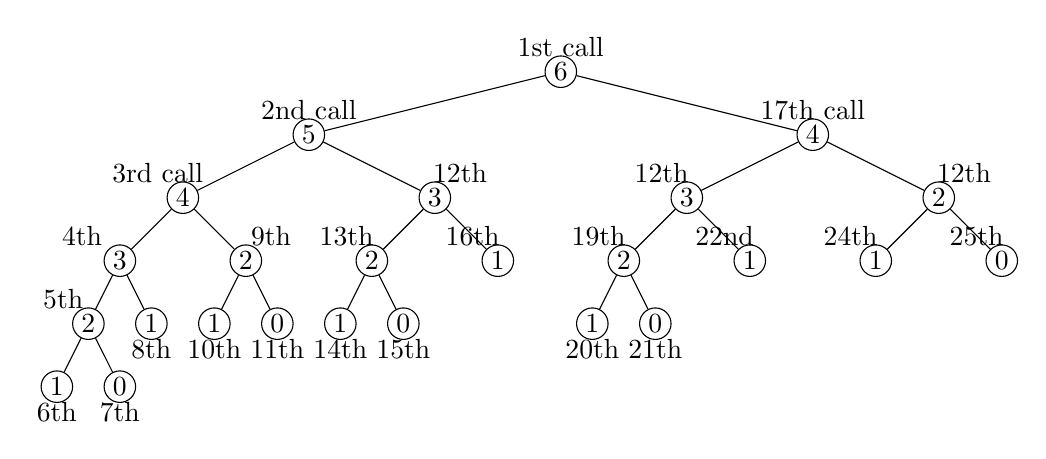
\begin{tikzpicture}[scale=0.8,place/.style={circle,draw, fill=white,inner sep=0pt,minimum size=4mm}]
    \node (A1)  at (0,0) [place] {6};
    \node (A1x)  at (0,0.4) {1st call};
    \node (B1)  at (-4,-1) [place] {5};
    \node (B1x)  at (-4, -0.6) {2nd call};
    \node (B2)  at (4, -1) [place] {4};
    \node (B2x)  at (4,-0.6) {17th call};

    \node (C1)  at (-6,-2) [place] {4};
    \node (C1x)  at (-6.4,-1.6) {3rd call};
    \node (C2)  at (-2, -2) [place] {3};
    \node (C2x)  at (-1.6,-1.6) {12th};
    \node (C3)  at (2,-2) [place] {3};
    \node (C3x)  at (1.6, -1.6) {12th};
    \node (C4)  at (6, -2) [place] {2};
    \node (C4x)  at (6.4, -1.6) {12th};

    \node (D1)  at (-7,-3) [place] {3};
    \node (D1x)  at (-7.6, -2.6) {4th};
    \node (D2)  at (-5,-3) [place] {2};
    \node (D2x)  at (-4.6, -2.6) {9th};
    \node (D3)  at (-3, -3) [place] {2};
    \node (D3x)  at (-3.4, -2.6) {13th};
    \node (D4)  at (-1, -3) [place] {1};
    \node (D4x)  at (-1.4, -2.6) {16th};
    \node (D5)  at (1, -3) [place] {2};
    \node (D5x)  at (0.6, -2.6) {19th};
    \node (D6)  at (3, -3) [place] {1};
    \node (D6x)  at (2.6, -2.6) {22nd};
    \node (D7)  at (5, -3) [place] {1};
    \node (D7x)  at (4.6, -2.6) {24th};
    \node (D8)  at (7, -3) [place] {0};
    \node (D8x)  at (6.6, -2.6) {25th};

    \node (E1)  at (-7.5,-4) [place] {2};
    \node (E1x)  at (-7.9, -3.6) {5th};
    \node (E2)  at (-6.5,-4) [place] {1};
    \node (E2x)  at (-6.5, -4.4) {8th};
    \node (E3)  at (-5.5, -4) [place] {1};
    \node (E3x)  at (-5.5, -4.4) {10th};
    \node (E4)  at (-4.5, -4) [place] {0};
    \node (E4x)  at (-4.5, -4.4) {11th};
    \node (E5)  at (-3.5, -4) [place] {1};
    \node (E5x)  at (-3.5, -4.4) {14th};
    \node (E6)  at (-2.5, -4) [place] {0};
    \node (E6x)  at (-2.5, -4.4) {15th};
    \node (E7)  at (0.5, -4) [place] {1};
    \node (E7x)  at (0.5, -4.4) {20th};
    \node (E8)  at (1.5, -4) [place] {0};
    \node (E8x)  at (1.5, -4.4) {21th};
    \node (F1)  at (-8,-5) [place] {1};
    \node (F1x)  at (-8, -5.4) {6th};
    \node (F2)  at (-7,-5) [place] {0};
    \node (F2x)  at (-7, -5.4) {7th};

    \draw (A1) -- (B1);
    \draw (A1) -- (B2);
    \draw (B1) -- (C1);
    \draw (B1) -- (C2);
    \draw (B2) -- (C3);
    \draw (B2) -- (C4);
    \draw (C1) -- (D1);
    \draw (C1) -- (D2);
    \draw (C2) -- (D3);
    \draw (C2) -- (D4);
    \draw (C3) -- (D5);
    \draw (C3) -- (D6);
    \draw (C4) -- (D7);
    \draw (C4) -- (D8);

    \draw (D1) -- (E1);
    \draw (D1) -- (E2);
    \draw (D2) -- (E3);
    \draw (D2) -- (E4);
    \draw (D3) -- (E5);
    \draw (D3) -- (E6);
    \draw (D5) -- (E7);
    \draw (D5) -- (E8);
    \draw (E1) -- (F1);
    \draw (E1) -- (F2);

    \end{tikzpicture}
    \caption{斐波纳契数列的递归计算的调用结构}
    \label{Fig:7_13Fib}
\end{figure*}
递归调用的执行顺序已经展示在插图之中;它非常类似于preorder序列。但是,结果累加
的序列(由+运算符连接)是postorder序列。我们已经看到一个更小的,更详细的例子的
活动帧在例\ref{Example:3_1ActivationFrames}。

对于图\ref{Fig:7_13Fib},我们假设25个顶点互不相同,即使很多是重复的标签,因为
每一个顶点并不仅仅对应它的标签,而且还对应这特定的函数调用。你可能想到这不是高
效率的计算Fibonacci数列的方法。你是对的。计算Fibonacci数列可以简化为一个对7个
顶点的图进行DFS,每一个顶点都有一个从0到6的唯一的标签。我们将在第
ref{Sec:Chapter:DynamicProgramming}章,\ref{Sec:10_2}小节重新回到这个话题。现在,
这个例子仅用来展示DFS和递归之间的联系。

\end{example}

因此,用递归解决许多有趣问题的逻辑结构就是对树的DFS遍历。树并不总是问题显式的一
部分,也不是现实的数据的结构的表现形式。下一个例子中,让我们看看著名的8皇后问题。

\begin{example}
棋盘上的8皇后

考虑放置8个皇后在棋盘上的问题,其中8个皇后不能相互攻击到;换句话说,没有一个皇后
能通过行,列,对角线碰到其他皇后。这个问题能不能完成也不是显而易见的。

\begin{figure*}[!t]
    \centering
    \begin{tikzpicture}[scale=0.6, place/.style={inner sep=0pt, font=\scriptsize, text width=8mm, text centered, below},
                                   script/.style={fill=white,inner sep=0pt, font=\scriptsize, text width=20ex, text centered, below}]
    \node (A1)  at (-1,0) [place] {Start};
    \node (B1)  at (-9,-2) [place] {(1,1)};
    \node (B2)  at (7, -2) [place] {(1,8)};
    \node (B3)  at (-6,-2) [place] {(1,2) \\ \vspace{-2ex}. \\ \vspace{-2ex}. \\ \vspace{-2ex}.};
    \node (B4)  at (-4,-2) [place] {(1,3) \\ \vspace{-2ex}. \\ \vspace{-2ex}. \\ \vspace{-2ex}.};
    \node (B5)  at (-2, -2) [place] {(1,4) \\ \vspace{-2ex}. \\ \vspace{-2ex}. \\ \vspace{-2ex}.};
    \node (B6)  at (0,-2) [place] {(1,5) \\ \vspace{-2ex}. \\ \vspace{-2ex}. \\ \vspace{-2ex}.};
    \node (B7)  at (2,-2) [place] {(1,6) \\ \vspace{-2ex}. \\ \vspace{-2ex}. \\ \vspace{-2ex}.};
    \node (B8)  at (4,-2) [place] {(1,7) \\ \vspace{-2ex}. \\ \vspace{-2ex}. \\ \vspace{-2ex}.};

    \draw (A1) -- (B1);
    \draw (A1) -- (B2);
    \draw (A1) -- (B3.north);
    \draw (A1) -- (B4.north);
    \draw (A1) -- (B5.north);
    \draw (A1) -- (B6.north);
    \draw (A1) -- (B7.north);
    \draw (A1) -- (B8.north);

    \node (C1)  at (-12.5,-4) [place] {(2,3)};
    \node (C2)  at (-10.8, -4) [place] {(2,4) \\ \vspace{-2ex}. \\ \vspace{-2ex}. \\ \vspace{-2ex}.};
    \node (C3)  at (-9.6,-4) [place] {(2,5) \\ \vspace{-2ex}. \\ \vspace{-2ex}. \\ \vspace{-2ex}.};
    \node (C4)  at (-8.4,-4) [place] {(2,6) \\ \vspace{-2ex}. \\ \vspace{-2ex}. \\ \vspace{-2ex}.};
    \node (C5)  at (-7.2, -4) [place] {(2,7) \\ \vspace{-2ex}. \\ \vspace{-2ex}. \\ \vspace{-2ex}.};
    \node (C6)  at (-5.5,-4) [place] {(2,8)};
    \node (C7)  at (3.4,-4) [place] {(2,1) \\ \vspace{-2ex}. \\ \vspace{-2ex}. \\ \vspace{-2ex}.};
    \node (C8)  at (4.6,-4) [place] {(2,2) \\ \vspace{-2ex}. \\ \vspace{-2ex}. \\ \vspace{-2ex}.};
    \node (C9)  at (5.8,-4) [place] {(2,3) \\ \vspace{-2ex}. \\ \vspace{-2ex}. \\ \vspace{-2ex}.};
    \node (C10)  at (7,-4) [place] {(2,4)};
    \node (C11)  at (8.2,-4) [place] {(2,5)  \\ \vspace{-2ex}. \\ \vspace{-2ex}. \\ \vspace{-2ex}.};
    \node (C12)  at (9.4,-4) [place] {(2,6) \\ \vspace{-2ex}. \\ \vspace{-2ex}. \\ \vspace{-2ex}.};

    \draw (B1) -- (C1.north);
    \draw (B1) -- (C2.north);
    \draw (B1) -- (C3.north);
    \draw (B1) -- (C4.north);
    \draw (B1) -- (C5.north);
    \draw (B1) -- (C6.north);
    \draw (B2) -- (C7.north);
    \draw (B2) -- (C8.north);
    \draw (B2) -- (C9.north);
    \draw (B2) -- (C10.north);
    \draw (B2) -- (C11.north);
    \draw (B2) -- (C12.north);

    \node (D1)  at (-14.3,-6) [place] {(3,5)};
    \node (D2)  at (-13.1,-6) [place] {(3,6) \\ \vspace{-2ex}. \\ \vspace{-2ex}.};
    \node (D3)  at (-11.9,-6) [place] {(3,7) \\ \vspace{-2ex}. \\ \vspace{-2ex}. \\ \vspace{-2ex}.};
    \node (D4)  at (-10.7,-6) [place] {(3,8) \\ \vspace{-2ex}. \\ \vspace{-2ex}. \\ \vspace{-2ex}.};
    \node (D5)  at (-7.3,-6) [place] {(3,1) \\ \vspace{-2ex}. \\ \vspace{-2ex}. \\ \vspace{-2ex}.};
    \node (D6)  at (-6.1,-6) [place] {(3,4) \\ \vspace{-2ex}. \\ \vspace{-2ex}. \\ \vspace{-2ex}.};
    \node (D7)  at (-4.9,-6) [place] {(3,5) \\ \vspace{-2ex}. \\ \vspace{-2ex}. \\ \vspace{-2ex}.};
    \node (D8)  at (-3.7,-6) [place] {(3,6) \\ \vspace{-2ex}. \\ \vspace{-2ex}. \\ \vspace{-2ex}.};
    \node (D9)  at (5.8,-6) [place] {(3,1) \\ \vspace{-2ex}. \\ \vspace{-2ex}. \\ \vspace{-2ex}.};
    \node (D10)  at (7,-6) [place] {(3,2) \\ \vspace{-2ex}. \\ \vspace{-2ex}. \\ \vspace{-2ex}.};
    \node (D11)  at (8.2,-6) [place] {(3,7) \\ \vspace{-2ex}. \\ \vspace{-2ex}. \\ \vspace{-2ex}.};

    \draw (C1) -- (D1.north);
    \draw (C1) -- (D2.north);
    \draw (C1) -- (D3.north);
    \draw (C1) -- (D4.north);
    \draw (C6) -- (D5.north);
    \draw (C6) -- (D6.north);
    \draw (C6) -- (D7.north);
    \draw (C6) -- (D8.north);
    \draw (C10) -- (D9.north);
    \draw (C10) -- (D10.north);
    \draw (C10) -- (D11.north);

    \node (E1)  at (-14.3,-8) [place] {(4,2)};
    \node (E2)  at (-11.9,-8) [place] {(4,7)};
    \node (E3)  at (-9.5,-8) [place] {(4,8)};
    \draw (D1) -- (E1.north);
    \draw (D1) -- (E2.north);
    \draw (D1) -- (E3.north);

    \node (F1)  at (-14.9,-10) [place] {$\underline{(5,4)}$};
    \node (F2)  at (-13.7,-10) [place] {$\underline{(5,8)}$};
    \node (F3)  at (-12.5,-10) [place] {(5,2)};
    \node (F4)  at (-11.3,-10) [place] {$\underline{(5,4)}$};
    \node (F5)  at (-10.1,-10) [place] {(5,3)};
    \node (F6)  at (-8.9,-10) [place] {$\underline{(5,4)}$};
    \draw (E1) -- (F1.north);
    \draw (E1) -- (F2.north);
    \draw (E2) -- (F3.north);
    \draw (E2) -- (F4.north);
    \draw (E3) -- (F5.north);
    \draw (E3) -- (F6.north);

    \node (G1)  at (-12.5,-12) [place] {(6,4)};
    \node (G2)  at (-10.1,-12) [place] {(6,4)};
    \node (H1)  at (-12.5,-14) [place] {$\underline{(7,6)}$};
    \node (H2)  at (-10.1,-14) [place] {$\underline{(7,6)}$};
    \draw (F3) -- (G1.north);
    \draw (F5) -- (G2.north);
    \draw (G1) -- (H1.north);
    \draw (G2) -- (H2.north);

    \node (S1)  at (-5,-10.5) [script] {$\underline{\mbox{下划线表示死路}}$ \\ 顶点上的标记表示皇后在棋盘上位置的坐标};
    \draw[step=1] (-3,-16) grid (5, -8);
    \node (S2)  at (-2.5,-8.5) [place] {Q};
    \node (S3)  at (-0.5,-9.5) [place] {Q};
    \node (S4)  at (1.5,-10.5) [place] {Q};
    \node (S5)  at (0.5,-12.5) [place] {Q};
    \node (S6)  at (-1.5,-11.5) [place] {Q};

    \end{tikzpicture}
    \caption{8皇后问题}
    \label{Fig:7_14EightQueen}
\end{figure*}

我们按如下的方式尝试:将一个皇后放在第一行第一列的方格中。然后继续将皇后放置在
第二行的未被占用的空格中,且该空格不能攻击到。重复之,直到8个皇后都在棋盘上。
或者下一空行中所有的空格都在攻击之下。如果后一种情况发生(例如图\ref{Fig:7_14EightQueen}
第第六行),就回到前一行,将皇后朝右移送移动到不被攻击到的位置,然后再放下一个。

这个问题中牵涉到的树是什么,我们在DFS中所做的事情如何对应?图\ref{Fig:7_14EightQueen}
展示了这颗树。每一个顶点(除了root)通过皇后在棋盘上的位置来标记。对于$1\leq
i \leq
8$,在第i层的顶点以第i行的位置来标记。第i层顶点$\nu$的孩子,是在第$i+1$行中不会被
攻击到的所有位置,是被从root到$\nu$的所有顶点表示的皇后攻击到;换句话说,孩子是
下一行中所有安全的位置。在树的术语中,8皇后问题的解是要找一条从root出发到叶子的
长度为8的路径。作为一个练习,你将为皇后问题写一个递归程序,递归调用的执行对应着
DFS。如果有一个解,图\ref{Fig:7_14EightQueen}展示的树只有一部分会被遍历到。(当DFS
用于8皇后这种问题时,也称为回溯搜索。)
\end{example}

\subsection{使用深度优先查找连同分量}\label{Sec:DFSOnUndirectedGraphs}
这一节发展了识别图的联通分量(或者对称有向图的强联通分量)的详细算法。本章中,
我们已经得出了大量的适用于所有DFS的实现细节。联通分量是与无向图关联的,但是无向图
的表示方式与对称有向图的表示方式相同,联通块在两种情况下是一样的。但是,DFS算法
(无向图上的)比在有向图上的的算法稍微简单一点。

令$G=(V,E)$是一个无向图,其中$n=|V|$,且$m=|E|$。对应的对称有向图有$2m$条有向边。
既然他们表示方法是一样的,我们将适用$G$表示这个对称有向图。复习一下,$G$的
\emph{联通分量}是最大的联通子图,也就是说,一个联通子图不在包含更大的联通子图
(定义\ref{Def:Connected_Component})。例如,图\ref{Fig:7_7}有三个联通分量。找到
联通分量的问题可以是用稍作修改的DFS解决。我们可以从任意顶点开始,做DFS以找到一个
分量中所有 的顶点(和边),然后如果还剩顶点,选择一个,继续重复之。

我们用\ref{Sec:OverViewofDFS}小节中的DFS概括。如果我们选择了一种糟糕的实现,算法
的各个部分都可能需要大量的工作量。循环需要找到所有与$\nu$相邻的$ws$(在边的正向)。
当然,我们应该用邻接表去表示图,这样我们就能便利$\nu$的list,;如果我们使用邻接
矩阵我们将不得不在循环中扫描每一个$w$。仔细考虑到算法,每一个邻接表将仅遍历一次。
我们将用一个局部变量来记录我们在邻接表中的位置。(这意味着,在遍历的任意时刻
有一个变量存储在帧堆栈中来跟踪我们在那些部分完成的邻接链表中的位置,如同
\ref{Sec:3_2_1}解释的。)

作为一个算法,DFS在两个层次上操作。在上层,或者包装层(dfsSweep),发现未探索的
顶点,并且未找到的为发现顶点初始化一个DFS。底层,调用dfs,递归的执行DFS的动作。

在dfsSweep中发现未探索的顶点来启动一个新的DFS的问题可以用类似dfs算法发现新的未探索
方法处理。我们可以从我们上次离开时候的顶点开始,而不必每次都从头到尾遍历数组。

当顶点的状态从“未探索到”转变到“探索的”,为了避免重复工作,甚至无法停止的搜索
记录是至关重要的。在有些应用中,当顶点完成处理时,也就是“完成时”,记录工作也是
重要的。这写记录对于算法分析来说也是非常有用的。因此我们采用一种三色系统来记录
顶点的状态。

\begin{definition}
顶点查找状态的三色代码

\emph{白色}表示顶点是未发现的。\emph{灰色}表示顶点是发现的,但是它的处理还没完成。
\emph{黑色}表示顶点是已经发现的,且它已经被处理完了。
\end{definition}

现在让我们将注意力转到联通分量问题的特定需要。如果按联通分量划分的图的分区需要
记录在后面要用的数据结构中,这个数据结构可以给每一个顶点或者边标记上数字,以表示
它属于哪一个分量。一个更复杂的选择是为每一个分量做一个独立的顶点或者边的链表。选择
何种方法取决于后面要用到何种类型的信息。

联通分量算法在后面显示。使用了一个DFS过程,使得实现是显式的。算法中的过程
connectedComponents对应了前面提到的通用的dfsSweep,参看\ref{Sec:OverViewofDFS}小节。
我们将图当作一个对称有向图,而不是一个无向图,在这个意义上,我们做一个有向的DFS。
无向图上的DFS遗留了一些额外的复杂性,这些复杂性对于寻找联通分量来说是没有必要的;
这些细节在\ref{Sec:DFSonUndirectedGraph}小节描述。

\begin{algorithm}
联通分量

{\textbf{\emph{输入:}}}邻接表的数组adjVertices表示一个对称有向图$G=(V,E)$,如同
我们在\ref{Sec:GraphRepresentationsAndDataStructures}描述的,$n$表示顶点的数量。
数组的索引是从$1, \cdots, n$。$G$也能解释为无向图。

{\textbf{\emph{输出:}}}数组cc,其中每一个元素表示一个顶点,元素的值表示顶点属于
那一个分量。联通分量的标识符是在分量中顶点的数量(其他的标识系统也是可行的)。
(调用者负责分配cc,过程负责填充cc。)

{\textbf{\emph{Remarks:}}}颜色的含义是$white=\mbox{未探索的}$,$gray=\mbox{活动的}$
$black=\mbox{完成的}$。过程ccDFS第三个和第四个参数都是顶层调用的$\nu$,但是他们有不同
的含义。第三个参数标明了当前要访问的顶点,但是在每一次递归调用中都会变。第四个参数
标明了联动分量的的标识,在递归调用中保持不改变。
\end{algorithm}

\begin{lstlisting}[language={Java},keywordstyle=\color{blue!70}, commentstyle=\color{red!50!green!50!blue!50}]
void connectedComponents(IntList[] adjVertices, int n,
    int[] cc)
    int[] color = new int[n+1];
    int v;
    `初始化所有顶点为白色`
    for(v=1; v<=n; v++)
        if( color[v] == white)
            ccDFS(adjVertices, color, v, v, cc);
    return;
void ccDFS(IntList[] adjVertices, int[] color, int v,
    int ccNum, int[] cc)
    int w;
    IntList remAdj;
    color[v] = gray;
    cc[v] = ccNum;
    remAdj = adjVertices[v];
    while(remAdj!= null)
        w = first(remAdj);
        if( color[w] == white)
            ccDFS(adjVertices, color, w, ccNum, cc);
        remAdj = rest(remAdj);
    color[v] = black;
    return;
\end{lstlisting}

\subsubsection{联通分量的分析}
算法connectedComponents所做的所有操作,包括调用ccDFS,显然是n的线性。在
$ccDFS(\ldots, \nu, \ldots)$,执行指令的数量与要遍历的邻接表的adjVertices[v]
的元素成比例,既然指令“remAdj = rest(remAdj)”每次\textbf{while}循环的执行
一次。既然邻接表仅仅被遍历一次,DFS复杂性,因此联通分量,是在$\Theta(n+m)$。
(通常$m\geq n$)\

邻接表结构使用的空间在$\Theta(n+m)$,但是算法输入的一部分。额外的空间被
$color$数组(n+1个条目)使用,另外递归可能引起活动帧堆栈增长到n,所以额外的
空间使用是$\Theta(n)$。


\subsubsection{联通分量的Remarks}
算法的输出是一个简单的数组cc,数组中包含了每一个元素联通分量的标识符(常使
用术语\emph{leader})。遍历一边数组cc的足够可以装配成一组链表,每一个链表仅包含
在一个联通分量中的顶点。同样的遍历一边adjVertices并参考cc,就足够装配出一套
链表,在每一个链表中包含一个联通分量中所有的边。这些可以在postprocessing步骤中
的步骤不会增加总的复杂性,所以只需要为基本的算法增加一点复杂性就可以裁剪出特定
的输出格式。

过程ccDFS不会对顶点做postorder处理(如果要做这种处理,应该是在语句"color[v]=black"
之前的代码)。这里有一个提示BFS也能简单的解决这个问题。

\subsection{DFS树}\label{Sec:DFS_Trees}
DFS树和DFS森林,在后面定义,对DFS算法提供了一种重要的深刻理解,有很多细微的区别。
算法\ref{Algo:DFS}将展示如何构造一颗DFS树。大多数的问题不需要构造DFS树,但是构造
一个DFS树将有助于分析。这里给出的DFS树的定义是适用于有向图的。尽管有向图中的中的
许多都适用于类似形式的无向图,但是依然有许多区别,所以无向图的定义延迟到
\ref{Sec:DFSonUndirectedGraph}小节.

\begin{definition}\label{Def:DFSTree_and_DFSForest}
DFS树,DFS森林

在一个有向图$G$的DFS过程中指向未发现的顶点(即白色顶点)的有唯一root的一组边称为
\emph{DFS搜索树}(有时候称为\emph{深度优先生成树depth-first spanning tree},也简称
为\emph{DFS树})。如果并不是所有的顶点都在以某个顶点开始的树中,则一个对$G$的完整的
遍历会生成多个树,合在一起称为\emph{DFS森林depth-first search forest}(有时称为
\emph{深度优先生成树depth-first spanning tree},也简称为\emph{DFS森林})。
\end{definition}

\begin{definition}\mbox{}\par

我们看到,如果$\nu$在从root到$\omega$的路径上,则顶点$\nu$在树中是$\omega$的\emph{祖先};
如果$\nu$是$\omega$的祖先,且$\nu\neq\omega$,则$\nu$称为$\omega$的\emph{真祖先}。
顶点$\nu$的最近的真祖先是$\nu$的\emph{父顶点}。如果$\nu$是$\omega$是(真)祖先,则
$\omega$是$\nu$的(真)子孙。
\end{definition}

\begin{definition}\mbox{}\par
有向图$G$的边分类的依据是,边是如何\emph{探索的}(在他们正向的遍历中)。
\begin{enumerate}
\item 如果$\omega$在$\nu\omega$的时刻是未探索的,则$\nu\omega$被称为\emph{树边},
而$\nu$变成$\omega$的父节点。

\item 如果$\omega$是$\nu$的祖先,则$\nu\omega$被称为\emph{回边}。(这种包含$\nu\nu$。)

\item 如果$\omega$是$\nu$的后代,则$\omega$被发现的点早于$\nu\omega$被探索的时刻,
则$\nu\omega$称为\emph{后代边}(另一个名字是\emph{前向边}或者\emph{frond})。

\item 如果$\omega$和$\nu$没有先祖或者后代关系,则$\nu\omega$被称为\emph{穿越边}。
\end{enumerate}
\end{definition}

\begin{example}\label{Example:7_11}
DFS树

让我们看看在例\ref{Example:DFS}Terry的旅程中边是如何被DFS引导分类的。Terry从$A$
开始(所以$A$是第一个DFS树的根),探索$B$,然后$C$,然后回溯到$B$,探索$D$。所以
边$AB$,$BC$和$BD$是树的边。现在Terry在D并遇到了第一个不是树的边。
\begin{tikzpicture}[scale=1.2,place/.style={circle,draw, fill=white,inner sep=0pt,minimum size=4mm}]
    \node (A1)  at (0,0) [place] {A};
    \node (B1)  at (1,-0.5) [place] {B};
    \node (C1)  at (1, -1.1) [place] {C};
    \node (D1)  at (2,0) [place] {D};
    \node (E1)  at (2,-1.1) [place] {E};
    \node (F1)  at (0, -1.1) [place] {F};
    \node (G1)  at (2.2, -0.5) [place] {G};
    \draw [double, ->] (A1) -- (B1);
    \draw [->] (A1) -- (C1);
    \draw [->] (A1) to [out=-70,in=70] (F1);
    \draw [very thick, ->] (B1) -- (C1);
    \draw [double, ->] (B1) -- (D1);
    \draw [dash pattern=on 3pt off 3pt, ->] (D1) -- (A1)  node[midway,sloped,above]{back};
    \draw [dash pattern=on 3pt off 3pt, ->] (D1) -- (C1) node[midway,sloped,below]{cross};
    \draw [->] (E1) -- (C1);
    \draw [->] (E1) to [out=90,in=240] (G1);
    \draw [->] (F1) to [out=110,in=-110] (A1);
    \draw [->] (F1) -- (C1);
    \draw [->] (G1) -- (D1);
    \draw [->] (G1) to [out=-100,in=60] (E1);
    \draw (2.3, 0) node[shape=diamond,draw, fill=black, minimum width=1mm, minimum height=1mm] {};

    \node (A2)  at (4,0) [place] {A};
    \node (B2)  at (5,-0.5) [place] {B};
    \node (C2)  at (5, -1.1) [place] {C};
    \node (D2)  at (6,0) [place] {D};
    \node (E2)  at (6,-1.1) [place] {E};
    \node (F2)  at (4, -1.1) [place] {F};
    \node (G2)  at (6.2, -0.5) [place] {G};
    \draw [very thick, ->] (A2) -- (B2);
    \draw [dash pattern=on 3pt off 3pt,->] (A2) -- (C2) node[midway,sloped,below]{descendant};
    \draw [->] (A2) to [out=-70,in=70] (F2);
    \draw [very thick, ->] (B2) -- (C2);
    \draw [very thick,->] (B2) -- (D2);
    \draw [dash pattern=on 3pt off 3pt, ->] (D2) -- (A2) node[midway,sloped,above]{back};
    \draw [dash pattern=on 3pt off 3pt, ->] (D2) -- (C2) node[midway,sloped,below,text width=3mm]{cross};
    \draw [->] (E2) -- (C2);
    \draw [->] (E2) to [out=90,in=240] (G2);
    \draw [->] (F2) to [out=110,in=-110] (A2);
    \draw [dash pattern=on 3pt off 3pt, ->] (F2) -- (C2);
    \draw [->] (G2) -- (D2);
    \draw [->] (G2) to [out=-100,in=60] (E2);
    \draw (3.7, 0) node[shape=diamond,draw, fill=black, minimum width=1mm, minimum height=1mm] {};

    \node (A3)  at (8,0) [place] {A};
    \node (B3)  at (9,-0.5) [place] {B};
    \node (C3)  at (9, -1.1) [place] {C};
    \node (D3)  at (10,0) [place] {D};
    \node (E3)  at (10,-1.1) [place] {E};
    \node (F3)  at (8, -1.1) [place] {F};
    \node (G3)  at (10.2, -0.5) [place] {G};
    \draw [very thick, ->] (A3) -- (B3);
    \draw [dash pattern=on 3pt off 3pt, ->] (A3) -- (C3) node[midway,sloped,below]{descendant};
    \draw [very thick, ->] (A3) to [out=-70,in=70] (F3);
    \draw [very thick, ->] (B3) -- (C3);
    \draw [very thick, ->] (B3) -- (D3);
    \draw [dash pattern=on 3pt off 3pt, ->] (D3) -- (A3)  node[midway,sloped,above]{back};
    \draw [dash pattern=on 3pt off 3pt, ->] (D3) -- (C3) node[midway,sloped,above]{cross};
    \draw [->] (E3) -- (C3);
    \draw [->] (E3) to [out=90,in=240] (G3);
    \draw [dash pattern=on 3pt off 3pt, ->] (F3) to [out=110,in=-110] (A3)  node[midway,sloped,below]{back};
    \draw [dash pattern=on 3pt off 3pt, ->] (F3) -- (C3)  node[midway,sloped,below]{cross};
    \draw [->] (G3) -- (D3);
    \draw [->] (G3) to [out=-100,in=60] (E3);
    \draw (7.7,0) node[shape=diamond,draw, fill=black, minimum width=1mm, minimum height=1mm] {};

    \end{tikzpicture}
双线标记了还没有被回溯的树的边,粗线标记了已经被回溯的树的边,细线标记了未探索的边,
虚线标记了不是树的边。在左边的图中,A是D的树的祖先,所以DA是一条\emph{back edge}.
但是C在树中既不是D的祖先也不是D的后代,所以DC是一条\emph{cross edge}.

中间的图展示了Terry从D回溯到B的以及从B回溯到A的情况。在AC 被探索的时候顶点C已经是
A在树中的祖先,;C已经被从其他的路由发现了。因此AC是\emph{descendant edge}(或者
成为\emph{forward edge} 或者frond)一个descendand 边总是是一条长的树的路径的快捷
路径。

左右边的图展示了DFS树完成时的情况。尽管Terry没有地方可去了,图的DFS还没有完成。

为了完成图的DFS,从E开始一个新的搜索。边EC到了一个完成顶点\footnote{译注:C已经
被访问过了}。C不能作为另外一个DFS树的顶点被再次访问,这一点是非常重要的。边EC划分为
cross edge;现在属于不同树的顶点没有祖先/后代关系。边EG是接着被考虑的边,它指向一个
未探索的顶点,所以它是一条树的边。接着GD指向另一个DFS树中的完成顶点,所以它是一条
cross边。边GE是黑的边,因为它指向当前DFS树中G的祖先。因此第二颗树有2个顶点和一条边,
它完成了DFS森林。(只有一个顶点没有边的树也是可能的:假设第一次DFS从顶点C空间开始。)
最后的DFS森林展示在图\ref{Fig:7_15DFStree}中,并且标注了所有的不是树的边。
\end{example}

\begin{figure*}[!t]
    \centering
    \begin{tikzpicture}[scale=2,place/.style={circle,draw, fill=white,inner sep=0pt,minimum size=4mm}]


    \node (A3)  at (8,0) [place] {A};
    \node (B3)  at (9,-0.5) [place] {B};
    \node (C3)  at (9, -1.1) [place] {C};
    \node (C4)  at (11, -1.1)  {To C};
    \node (D3)  at (10,0) [place] {D};
    \node (D4)  at (11.6,0) {TO D};
    \node (E3)  at (12,-1.1) [place] {E};
    \node (F3)  at (8, -1.1) [place] {F};
    \node (G3)  at (12.2, -0.5) [place] {G};
    \draw [very thick, ->] (A3) -- (B3);
    \draw [dash pattern=on 3pt off 3pt, ->] (A3) -- (C3) node[midway,sloped,below]{descendant};
    \draw [very thick, ->] (A3) to [out=-70,in=70] (F3);
    \draw [very thick, ->] (B3) -- (C3);
    \draw [very thick, ->] (B3) -- (D3);
    \draw [dash pattern=on 3pt off 3pt, ->] (D3) -- (A3)  node[midway,sloped,above]{back};
    \draw [dash pattern=on 3pt off 3pt, ->] (D3) -- (C3) node[midway,sloped,above]{cross};
    \draw [dash pattern=on 3pt off 3pt, ->] (E3) -- (C4) node[midway,sloped,above]{cross};
    \draw [very thick, ->] (E3) to [out=90,in=240] (G3);
    \draw [dash pattern=on 3pt off 3pt, ->] (F3) to [out=110,in=-110] (A3)  node[midway,sloped,below]{back};
    \draw [dash pattern=on 3pt off 3pt, ->] (F3) -- (C3)  node[midway,sloped,below]{cross};
    \draw [dash pattern=on 3pt off 3pt, ->] (G3) -- (D4) node[midway,sloped,above]{cross};
    \draw [dash pattern=on 3pt off 3pt, ->] (G3) to [out=-100,in=60] (E3) node[midway,sloped,below]{back};

    \end{tikzpicture}
    \caption{粗线边展示了例\ref{Example:DFS}和例\ref{Example:7_11}中图的DFS森林。虚线边不是树的边,做了对应的标记。}
    \label{Fig:7_15DFStree}
\end{figure*}

边的分类非常依赖于邻接表中顶点的顺序(参看练习7.4)。注意cross边的头和尾分别属于两个不同
的树。不同类型边之间的区别在许多DFS的应用中都非常重要——特别是在\ref{Sec:7_5StronglyConnectedComponentsofDirgraph}
节和\ref{Sec:7_7BiConnectedComponentsofUndirgraph}节。

\subsection{通用DFS骨架}\label{Sec:7_4_4}
DFS算法提供了许多优美高效的算法。如我们在几个例子中看到的,一个DFS算法遭遇一个顶点数次:
当顶点第一次被发现并成为DFS树的一部分时,之后可能多次\emph{回溯到}这个顶点的并要在DFS树
分枝出新的子树时,最后这些遭遇之后,当搜索\emph{从顶点回溯}并不在再次穿过它的时候。依赖于
要解决的问题,一个算法会在遍历中的不同步骤遭遇顶点时采取不同的处理。许多算法也同时对边做
处理——可能是每一条边,或者仅仅是DFS树中的边,或者可能对不同的边做不同的计算。下面的骨架
算法明确的展示了每一种边可以做啥操作,每一种遭遇顶点的时刻做的操作。

\begin{algorithm}\label{Algo:SkeletonDirectGraphDFS}
有向图的DFS骨架(DFS Skeleton)

{\textbf{\emph{输入:}}}邻接表的数组adjVertices表示一个对称有向图$G=(V,E)$,如同
我们在\ref{Sec:GraphRepresentationsAndDataStructures}描述的,$n$表示顶点的数量。
数组的索引是从$1, \cdots, n$。应用需要的其他参数。

{\textbf{\emph{输出:}}}返回值依赖于具体应用。返回值可能是千变万化的;int只是一个
例子。

{\textbf{\emph{Remarks:}}}这个估计也是足够用于有些忽略了非树边无向图问题,但是参考
算法\ref{Algo:SkeletonUndirectGraphDFS}。颜色的含义是白色=未发现的,灰色=活动的,
黑色=完成的。

\end{algorithm}

\begin{figure}
\begin{lstlisting}[language={Java},keywordstyle=\color{blue!70}, commentstyle=\color{red!50!green!50!blue!50}]
void dfsSweep(IntList[] adjVertices, int n,...)
{
    int ans;
    `分配颜色数组初始化所有顶点为白色`
    foreach vertex v in G,`以某种顺序:`
        if( color[v] == white)
            int vAns = dfs(adjVertices, color, v,...);
            `处理 vAns`
        // `继续循环`
    return ans;
}

int dfs(IntList[] adjVertices, in[] color, int v,...)
{
    int w;
    IntList remAdj;
    int ans;
1.  color[v] = gray;
2.  Preorder processing of vertex v
3.  remAdj = adjVertices[v];
4.  while(remAdj != null)
    {
5.      w = first(remAdj);
6.      if( color[w] == white)
        {
7.          `试探性处理树边vw`
8.          int wAns = dfs(adjVertices, color, w,...);
9.          `回溯处理树边vw,使用wAns`
        }
        else
11.         `检查非树边`
12.     remAdj = rest(remAdj)
    }
    `Postorder 处理顶点v, 包括最后的ans的计算`
14. color[v] = black;
15. return ans;
}
\end{lstlisting}
\end{figure}

对于有些应用程序,程序可能在搜索的途中就被解决了。结束的条件应该在第9行检查,或者
第11行。推荐使用一个\textbf{break}来体检推出\textbf{while}循环,所以postorder processing
包含设置颜色到黑色。


\begin{example}
将DFS skeleton用于联通分量问题

为了展示骨架的多才多艺,让我们使用它来重新解决连同分量的问题。
\begin{enumerate}
\item 传递数组cc作为dfsSweep得一个额外的参数。这个数组将被算法填上连同分量的数字。
\item 增加第4个参数ccNum,第5个参数cc,到dfs。当dfsSweep调用dfs时,在dfsSweep中将
第4个参数设置为v,它同样是第3个参数,设置第5个参数为cc。
\item 在dfs递归调用,使用同样的ccNum和cc。
\item 对于preorder processing(骨架的第2行),插入一句“cc[v]=ccNum.”
\end{enumerate}
有了这些改变——一行新的代码,一些额外的参数,我们已经通用目的的骨架具体化来解决
连同分量的问题。我们将在本章剩下的部分以及练习中,看到许多使用骨架的例子。
\end{example}

\subsection{DFS的结构}
在有些DFS的应用中,我们可能需要知道当前DFS树中从root到当前顶点$\nu$有那些顶点,就是
说那些被访问了。他们都是灰色顶点,在栈帧中以$\nu$为参数的调用之下(也就是说接近活动
帧树的root)。对于有些算法,我们需要知道从第一次到最后一次遭遇顶点的顺序,或者两个
遭遇顶点之间的关系。一个简单,有效的办法是在两个数组中跟踪这些关系,dicoverTime和
finishTime。一个全局的整数变量time在开始初始化为0,每当一个顶点的颜色变化就增加time。

\begin{definition}\label{Def:DFSTerminology}
DFS 术语

当$\nu$的颜色是白色时,我们称它是\emph{未发现的}。当color[v]变成灰色时,当前的time记录在
discoverTime[v]中(在骨架的第2行);现在$\nu$是\emph{活动的}。当color[v]编程黑色时,当前
的time记录在finishTime[v](估计的第13行),此时$\nu$是\emph{完成的}。顶点$\nu$的
\emph{active interval},标记为$active(v)$,定义为如下整数区间:
\begin{displaymath}
active(\nu) = discoverTime[v], \ldots, finishTime[v]
\end{displaymath}
包括两个端点,所以$\nu$恰好在活动区间之内变灰色。Time的最后的值应该是2n,如果整个图都被
遍历到的话。
\end{definition}

我们可以在DFS骨架中插入代码来计算dicovery和finishing times,以及DFS森林的“construct”。
我们称之为\emph{DFS Trace}算法。即使一个使用DFS骨架的算法没有包含这些代码,为了分析的
目的我们可以使用这些如果插入了算法就可以得到的值。

\begin{algorithm}\label{Algo:DFS_Trace}
DFS Trace

{\textbf{\emph{输入:}}} 与算法\ref{Algo:SkeletonDirectGraphDFS}有同样的输入,增加全局数组
discoverTime,finishingTime,parent;以及算据计数器time。

{\textbf{\emph{输出:}}}前面提到的全局数组被填充。算法的返回类型可以被改成void。parent数
组以in-tree的方式存储dfs森林。其他的数组的含义参见定义\ref{Def:DFSTerminology}。

{\textbf{\emph{Strategy}}}将算法\ref{Algo:SkeletonDirectGraphDFS}的DFS骨架改成如下:
\begin{enumerate}
\item 在dfsSweep初始化 time 为0
\item 在dfsSweeo中,调用dfs(在“if”之后)之前插入“parent[v]=-1”
\item 在dfs中,递归调用dfs之前(“if”之后)插入“parent[w]=v”
\item 在骨架的preorder处理(第2行),插入
      \begin{displaymath} time++; discoverTime[v] = time; \end{displaymath}
      (是是$\nu$变成活动的时刻。)
\item 在骨架的postorder(第13行),插入
      \begin{displaymath} time++; finishTime[v] = time; \end{displaymath}
      (这是$\nu$变成不活动的时刻。)
\end{enumerate}

\end{algorithm}

\begin{figure*}[!t]
    \centering
    \begin{tikzpicture}[scale=2,place/.style={circle,draw, fill=white,inner sep=0pt,minimum size=4mm}]

XX


    \end{tikzpicture}
    \caption{DFS trace算法在例\ref{}的图上的进展。双线是还没有被回溯到的树的边,
            所以他们只想灰色的顶点。粗线是已经被回溯的树的边,所以他们指向黑色
            的顶点。d/f表示了顶点的发现和完成时间。两颗dfs树被构建出来。不同的
            顶点顺序可以产生不同的trace。}
    \label{Fig:7_16}
\end{figure*}

图\ref{Fig:7_16}展示了一个算法\ref{Algo:DFS_Trace}的例子。根据定义\ref{Def:DFSTerminology}
的定义,每个顶点\emph{活动}的区间,以d/f的形式展示,这里d是顶点发现的时间,f是顶点
完成的时间。这些区间有有趣的重要的关系,对于每一个顺序,DFS森林(定义\ref{Def:DFSTree_and_DFSForest})
中顶点的相关位置都是。

\begin{figure*}[!t]
    \centering
    \begin{tikzpicture}[scale=2,place/.style={circle,draw, fill=white,inner sep=0pt,minimum size=4mm}]

XX


    \end{tikzpicture}
    \caption{图\ref{Fig:7_16}中DFS森林的\emph{活动}区间}
    \label{Fig:7_17}
\end{figure*}

\begin{definition}
嵌套\emph{活动}区间

对于图\ref{Fig:7_16}的DFS森林的\emph{活动}区间在图\ref{Fig:7_17}。顶点A是一颗DFS树的
根,E是
\end{definition}


\subsection{有向无环图}
\emph{有向无环图Directed acyclic graphs}(\emph{DAGs})是重要的特殊的有向图。如同它的
名字暗示的,一个DAG可以是任意有向图,只要它没有图。有向无环图之所以重要,有两个主要的
原因:
\begin{enumerate}
\item 许多问题可以自然的以DAG的术语来表示,例如日程安排问题。在日程安排问题中经常需要
考虑特定的任务必须在有些任务完成之后才能开始。任务依赖上的环将意味着死锁\emph{deadlock}:
环中没有任务能够开始。
\item 许多在一般有向图上的问题在DAGs上更容易解决——也就是说更有效率。这个差别可以足够
大到指数时间vs.线性时间。我们将在提到这些问题的通用版本时详细描述。
\end{enumerate}

同样的,我们将在\ref{Sec:7_5StronglyConnectedComponentsofDirgraph}节中看到每一个一般
有向图都与特定的有向无环图相关联,称为\emph{condensation graph}。

有向无环图代表了它的顶点之间的数学上的partial order。无论边$\nu\omega$在那里,我们都可以
将它解释为顶点之间的关系$\nu<\omega$。如果有从$\nu$到$\omega$有向路径,我们也可以通过
关系的传递性将它解释为$\nu<\omega$。(图中所有的边也可以解释为$\nu>\omega$。我们只要在图
中保持一致就行。)一个order(或者partial order)关系是不允许包含环的。我们将看到order的
解释在日程安排问题中是非常有用的。

在这一小节中我们将学习两个DAGs的应用:拓扑顺序和关键路径。

\subsubsection{拓扑顺序}
当考虑有向图上的一些问题时,你可能会问自己,“如果我能画出这个图,并且所有的边都从左到右,
这会帮助我解决问题吗?”当然,如果图有一个环,这显然是不可能的。但是如果有向图没有环——
一个DAG——则我们将看到这样安排顶点是可能的。找到这样一种安排就是
\emph{拓扑排序问题topological ordering}。

\begin{definition}
拓扑顺序 topological order

令$G=(V,E)$是一个有$n$个顶点的有向图。图$G$的拓扑顺序是
\end{definition}

\begin{figure*}[!t]
    \centering
    \subfloat{
        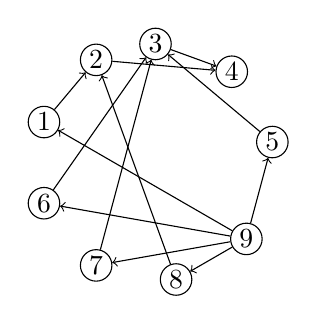
\begin{tikzpicture}[scale=1,place/.style={circle,draw, fill=white,inner sep=0pt,minimum size=4mm}]
            \node[name=s,shape=circle, minimum size=30mm] {};
            \draw[shift=(s.160)]node[name=x1,place] {1};
            \draw[shift=(s.120)]node[name=x2,place] {2};
            \draw[shift=(s.90)]node[name=x3,place] {3};
            \draw[shift=(s.50)]node[name=x4,place] {4};
            \draw[shift=(s.10)]node[name=x5,place] {5};
            \draw[shift=(s.200)]node[name=x6,place] {6};
            \draw[shift=(s.240)]node[name=x7,place] {7};
            \draw[shift=(s.280)]node[name=x8,place] {8};
            \draw[shift=(s.320)]node[name=x9,place] {9};

            \draw [->] (x1) -- (x2);
            \draw [->] (x2) -- (x4);
            \draw [->] (x3) -- (x4);
            \draw [->] (x5) -- (x3);
            \draw [->] (x6) -- (x3);
            \draw [->] (x7) -- (x3);
            \draw [->] (x8) -- (x2);
            \draw [->] (x9) -- (x7);
            \draw [->] (x9) -- (x8);
            \draw [->] (x9) -- (x1);
            \draw [->] (x9) -- (x5);
            \draw [->] (x9) -- (x6);
        \end{tikzpicture}
    }
    \hfil
    \subfloat{
        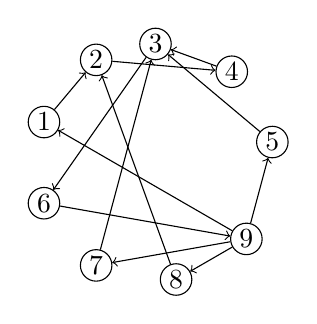
\begin{tikzpicture}[scale=1,place/.style={circle,draw, fill=white,inner sep=0pt,minimum size=4mm}]
            \node[name=s,shape=circle, minimum size=30mm] {};
            \draw[shift=(s.160)]node[name=x1,place] {1};
            \draw[shift=(s.120)]node[name=x2,place] {2};
            \draw[shift=(s.90)]node[name=x3,place] {3};
            \draw[shift=(s.50)]node[name=x4,place] {4};
            \draw[shift=(s.10)]node[name=x5,place] {5};
            \draw[shift=(s.200)]node[name=x6,place] {6};
            \draw[shift=(s.240)]node[name=x7,place] {7};
            \draw[shift=(s.280)]node[name=x8,place] {8};
            \draw[shift=(s.320)]node[name=x9,place] {9};

            \draw [->] (x1) -- (x2);
            \draw [->] (x2) -- (x4);
            \draw [->] (x3) -- (x6);
            \draw [->] (x4) -- (x3);
            \draw [->] (x5) -- (x3);
            \draw [->] (x6) -- (x9);
            \draw [->] (x7) -- (x3);
            \draw [->] (x8) -- (x2);
            \draw [->] (x9) -- (x7);
            \draw [->] (x9) -- (x8);
            \draw [->] (x9) -- (x1);
            \draw [->] (x9) -- (x5);
        \end{tikzpicture}
    }
    \caption{两个有向图,哪一个是无环的呢?}
    \label{Fig:7_18}
\end{figure*}

图\ref{Fig:7_18}展示的两个图,只有一个是无环的。邀请读者

\subsubsection{关键路径分析}

\subsubsection{有向无环图总结}

\section{有向图的强连通分支}\label{Sec:7_5StronglyConnectedComponentsofDirgraph}
\begin{definition}\label{Def:CondensationGraph}
Condensation graph

令
\end{definition}

\section{无向图的深度优先查找}\label{Sec:DFSonUndirectedGraph}
\begin{algorithm}\label{Algo:SkeletonUndirectGraphDFS}
无向图的DFS骨架(DFS Skeleton)
\end{algorithm}

\section{无向图的二连通分支}\label{Sec:7_7BiConnectedComponentsofUndirgraph}
在\ref{Sec:GraphDefinitionsAndRepresentations}节,我们提出了这些问题:
\begin{enumerate}
\item 如果一个城市的机场因为坏天气而关闭了,你仍然能在其他的任意两个城市之间飞行吗?
\item 如果网络中一台计算机崩溃了,消息仍然能在其他的任意两台网络中计算机之间传递吗?
\end{enumerate}
本节中明我们仅考虑无向图。作为一个图问题:

\begin{problem}\vspace{1ex}
如果任一顶点(与之相关联的边)从连通图中移除了,剩下的子图仍然是连通的吗?
\end{problem}
这个问题在代表通信或运输网络的图中是非常重要的。如果移除之后就使得图不在连通,
找出这些顶点也是很重要的。本节的目的就是找到有效的算法来回答这些问题。这个算法是
由R.E.Tarjan发现的,这个算法也是早期体现出深度优先查找的强大威力的算法。

\subsection{关节顶点和二连通分支}
我们从建立一些技术和基本属性开始。
\begin{definition}
二连通分支

连通无向图G是二连通的,当移除它的任一顶点以及与顶点相连的边之后,图仍然是连通的。

无向图的一个\emph{二连通分支}(简写为bicomponent)是最大的二连通子图,就是说,
不被更大的二连通自图所包含。
\end{definition}

显然,移除一个关节顶点会留下一个不连通的图,所以一个连通图是\emph{二连通}的,
当且仅当它没有关节顶点。观察这一点,尽管二连通分支将边划到不相交集合,但是并
不严格得划分顶点;有些顶点在多个分支里面。(那些顶点是?)
